% \appendix
\appendix
\chapter{Appendices}\label{chap:Appendices}
\renewcommand{\thesection}{\Alph{section}}
% \section{}\label{ap:MChyperparams}
% \begin{table}[htb!]
%     \centering
%     \caption{Table displaying single layer model hyperparameters fitted to Monte Carlo datasets of each refractive index (black) with available literature values (blue).}
%     \begin{tabular}{|cc|cc|c|cc|}
%         \hline
%         \multirow{2}{*}{Model} & \multirow{2}{*}{Parameter} & \multicolumn{5}{c|}{Refractive index} \\
%          & & \multicolumn{2}{c|}{1.33} & 1.35 & \multicolumn{2}{c|}{1.44} \\
%         \hline
%         \multirow{6}{*}{Yudovsky 2009} & $M_1$ & \multicolumn{2}{c|}{-0.0253} & -0.0257 & -0.0254 & \textcolor{blue}{-0.0247} \\
%         & $M_2$ & \multicolumn{2}{c|}{0.0166} & 0.0159 & 0.0135 & \textcolor{blue}{0.0137} \\
%         & $M_3$ & \multicolumn{2}{c|}{2.873} & 2.873 & 2.873 & \textcolor{blue}{2.873} \\
%         & $M_4$ & \multicolumn{2}{c|}{1.64} & 1.64 & 1.64 & \textcolor{blue}{1.64} \\
%         & $M_5$ & \multicolumn{2}{c|}{0.0123} & 0.0124 & 0.0120 & \textcolor{blue}{0.0116} \\
%         & $M_6$ & \multicolumn{2}{c|}{1.02} & 1.02 & 1.02 & \textcolor{blue}{1.02} \\
%         \hline 
%         \multirow{3}{*}{Jacques 1999} & $M_1$ & 7.0188 & \textcolor{blue}{6.3744} & 7.1185 & \multicolumn{2}{c|}{7.0438} \\
%         & $M_2$ & 0.2464 & \textcolor{blue}{0.35688} & 0.2750 & \multicolumn{2}{c|}{0.6902} \\
%         & $M_3$ & 4.2241 & \textcolor{blue}{3.4739} & 4.2571 & \multicolumn{2}{c|}{4.1449} \\
%         \hline
%         \multirow{3}{*}{Modified Beer-Lambert} & $M_1$ & \multicolumn{2}{c|}{0.283} & 0.308 & \multicolumn{2}{c|}{0.256} \\
%         & $M_2$ & \multicolumn{2}{c|}{0.009} & 0.008 & \multicolumn{2}{c|}{0.014} \\
%         & $M_3$ & \multicolumn{2}{c|}{0.203} & 0.311 & \multicolumn{2}{c|}{0.274} \\
%         \hline
%     \end{tabular}
%     \label{tb:fittedmodelparams}
% \end{table}
% \FloatBarrier
% 
% \section{}\label{ap:badYudovsky}
\section{Investigating single-layer models}
\begin{figure}[htb!]
    \centering
    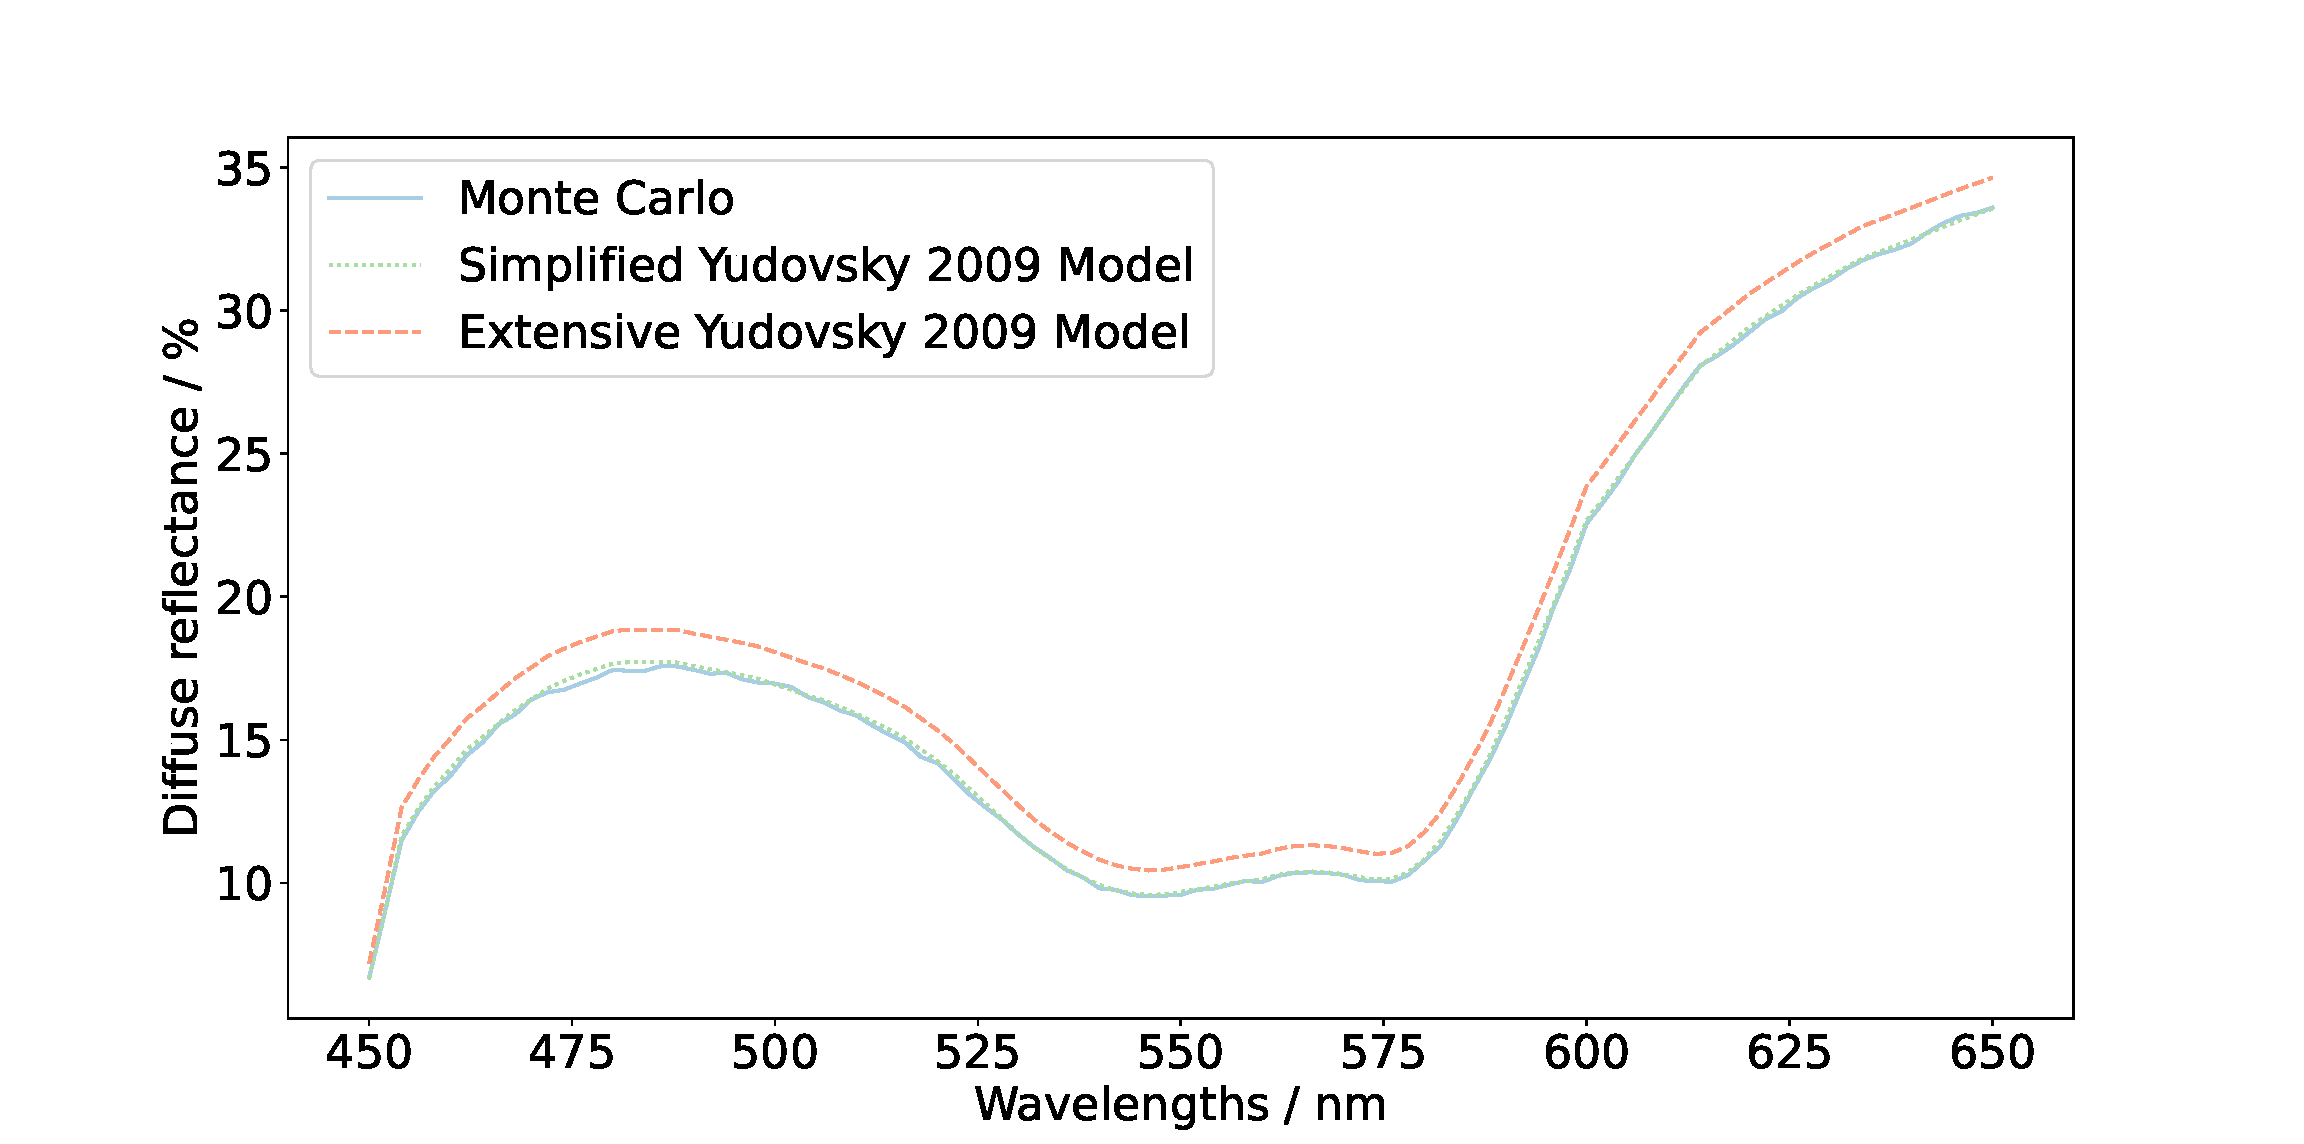
\includegraphics[width=0.65\textwidth]{Figure_A1}
    \caption{Example of difference in forwards model similarity to Monte Carlo simulation (blue solid) between the literature extensive Yudovsky 2009 (red dashed) and simplified Yudovsky 2009 (green dotted) models using ground truth variables for a refractive index of 1.44.}
 \label{fig:badYudovsky}
\end{figure}
\FloatBarrier

% \section{}\label{ap:MCforwardsr}
% \begin{figure}[htb!]
%     \centering
%     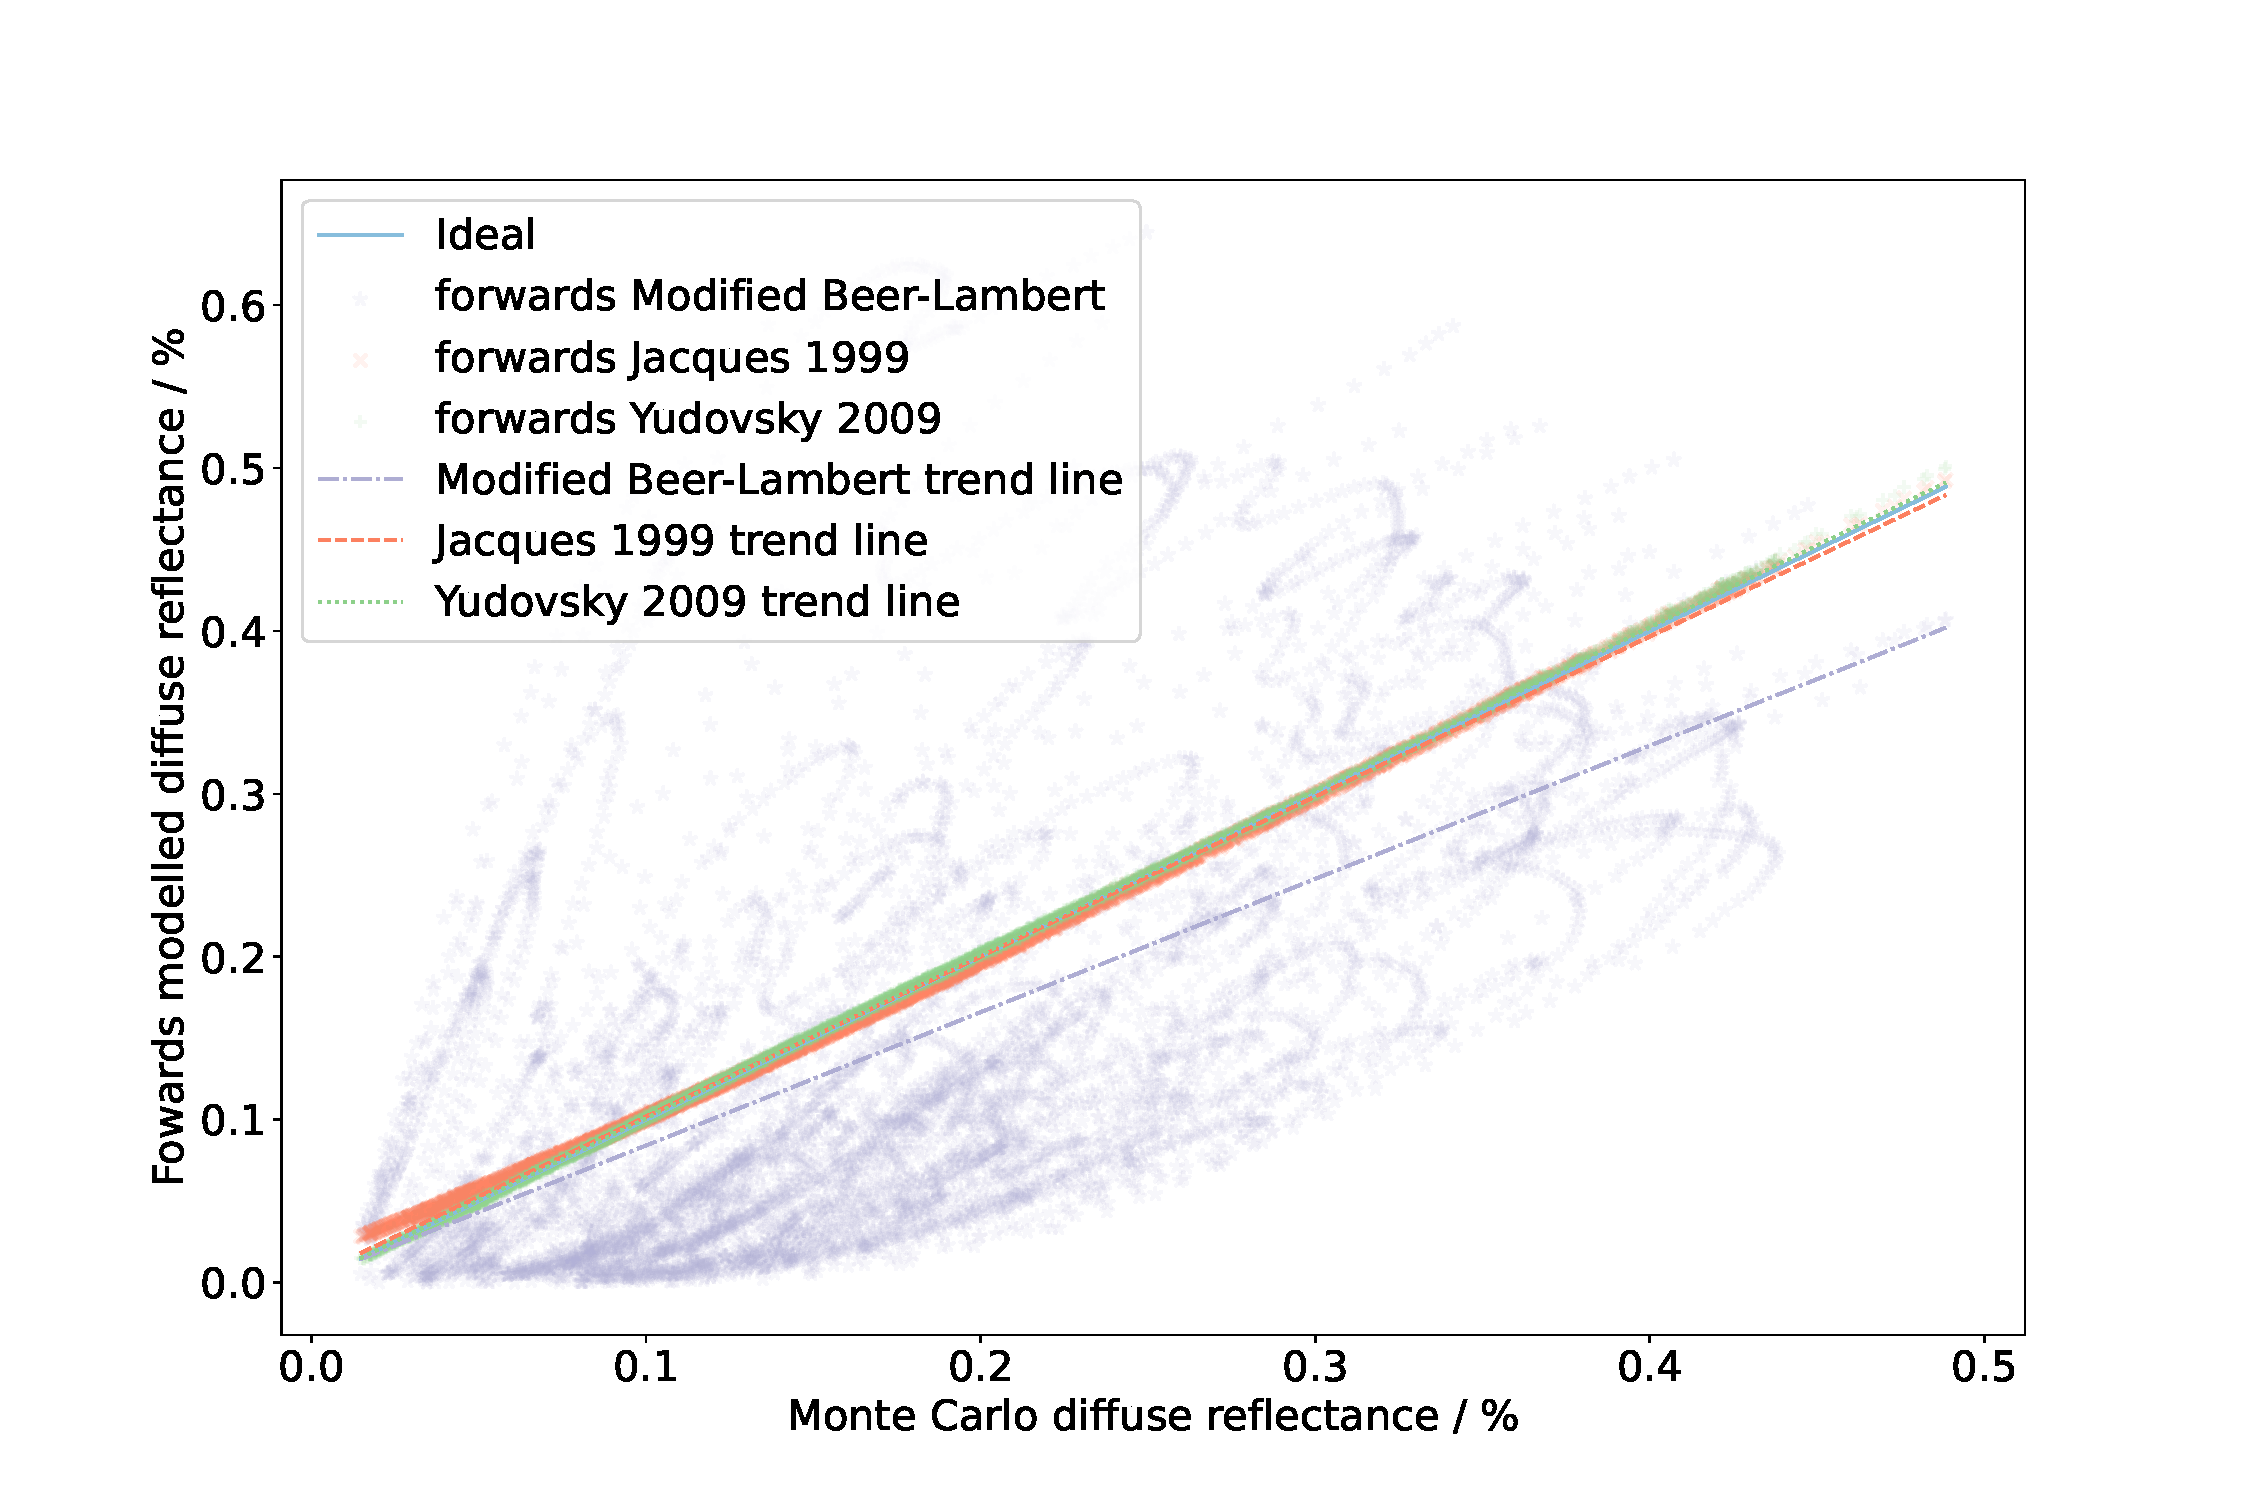
\includegraphics[width=0.7\textwidth]{forwards_v_MC_1.44.pdf}
%     \caption{Regression lines between the Monte Carlo simulated spectra and the analytical models: Yudovsky 2009 (green dotted), Jacques 1999 (red dashed), and Modified Beer-Lambert (orange dot-dashed) for a refractive index of 1.44.}
%  \label{fig:forwardsregressionMC}
% \end{figure}
% \FloatBarrier

% \section{}\label{ap:MCfullinverseparams}
\begin{table}[htb!]
    \centering
    \caption{The gradient $m$, offset $c$, Pearson $r$, and $p$ values of the linear regression line between the fitted tissue parameters and their ground truth displayed with their median (inter-quartile range) absolute percentage errors $APE$. This is shown for each variable and for each refractive index dataset when extracted by fitting Yudovsky 2009 (Y), Jacques 1999 (J), or Modified Beer-Lambert (BL) to the Monte-Carlo dataset. All presented to 3s.f.}
    \begin{tabular}{|ccc|ccccc|}
        \hline
        Parameter & Model & Refractive & $m$ & $c$ & $r$ & $p$ & $APE$ \\
        & & index & (ideal =1) & (ideal = 0) & (ideal = 1) & (ideal = 0) & (\%)\\
        \hline
        % \multicolumn{3}{|c|}{Ideal} & 1 & 0 & 1 & 0 & dependent on variable \\
        % \hline
        \multirow{9}{*}{$StO_2$} & \multirow{3}{*}{Y} & 1.33 & 1.00 & -0.373 & 1.00 & 2.39$\times 10^{-150}$ & 1.23 (3.01) \\
        & & 1.35 & 0.999 & 0.0672 & 1.00 & 4.93$\times 10^{-149}$ & 0.815 (2.10) \\
        & & 1.44 & 0.999 & -0.074 & 1.00 & 4.87$\times 10^{-153}$ & 0.913 (1.92) \\
        \cline{2-8}
        & \multirow{3}{*}{J} & 1.33 & 1.00 & 1.733 & 0.979 & 1.44$\times 10^{-69}$ & 3.40 (9.43) \\
        & & 1.35 & 1.03 & 1.03 & 0.980 & 2.18$\times 10^{-70}$ & 3.97 (12.9) \\
        & & 1.44 &  1.04 & 0.207 & 0.986 & 1.64$\times 10^{-77}$ & 2.21 (4.97) \\
        \cline{2-8}
        & \multirow{3}{*}{BL} & 1.33 & 0.712 & 1.56 & 0.855 & 1.17$\times 10^{-29}$ & 39.4 (38.5) \\
        & & 1.35 & 0.679 & 3.92 & 0.838 & 3.87$\times 10^{-30}$ & 33.3 (31.4) \\
        & & 1.44 & 0.766 & -2.73 & 0.838 & 1.70$\times 10^{-27}$ & 43.0 (49.8) \\
        \hline
        \multirow{9}{*}{$f_{blood}$} & \multirow{3}{*}{Y} & 1.33 & 0.976 & -0.0206 & 0.980 & 2.76$\times 10^{-70}$ & 5.74 (6.19) \\
        & & 1.35 & 0.962 & 0.0365 & 0.975 & 8.29$\times 10^{-66}$ & 4.58 (6.98) \\
        & & 1.44 & 0.927 & 0.152 & 0.982 & 3.60$\times 10^{-73}$ & 5.68 (6.08) \\
        \cline{2-8}
        & \multirow{3}{*}{J} & 1.33 & 1.17 & 0.187 & 0.915 & 2.21$\times 10^{-40}$ & 9.51 (28.7) \\
        & & 1.35 & 1.16 & 0.167 & 0.912 & 9.18$\times 10^{-40}$ & 11.0 (20.1) \\
        & & 1.44 & 1.15 & 0.141 & 0.928 & 1.10$\times 10^{-43}$ & 7.26 (16.2) \\
        \cline{2-8}
        & \multirow{3}{*}{BL} & 1.33 & 0.487 & 0.431 & 0.641 & 7.16$\times 10^{-13}$ & 46.4 (28.2) \\
        & & 1.35 & 0.461 & 0.478 & 0.575 & 3.99$\times 10^{-10}$ & 45.8 (41.8) \\
        & & 1.44 & 0.339 & 0.652 & 0.582 & 2.05$\times 10^{-10}$ & 49.6 (32.2) \\
        \hline
        \multirow{9}{*}{$a$} & \multirow{3}{*}{Y} & 1.33 & 0.948 & 0.145 & 0.993 & 2.58$\times 10^{-93}$ & 5.06 (5.92) \\
        & & 1.35 & 0.968 & -0.192 & 0.995 & 4.71$\times 10^{-102}$ & 4.05 (5.57) \\
        & & 1.44 & 1.05 & -2.59 & 0.992 & 1.67$\times 10^{-89}$ & 3.90 (4.73) \\
        \cline{2-8}
        & \multirow{3}{*}{J} & 1.33 & 0.909 & 7.23 & 0.952 & 4.13$\times 10^{-52}$ & 7.09 (22.0) \\
        & & 1.35 & 0.929 & 5.72 & 0.966 & 3.04$\times 10^{-59}$ & 9.16 (16.2) \\
        & & 1.44 & 0.934 & 5.88 & 0.959 & 1.05$\times 10^{-55}$ & 4.54 (15.3) \\
        \cline{2-8}
        & \multirow{3}{*}{BL} & 1.33 & -0.197 & 74.7 & -0.554 & 2.23$\times 10^{-9}$ & 63.8 (133) \\
        & & 1.35 & -0.142 & 73.1 & -0.448 & 2.89$\times 10^{-6}$ & 103 (206) \\
        & & 1.44 & -0.488 & 78.1 & -0.706 & 2.28$\times 10^{-16}$ & 40.0 (114) \\
        \hline
        \multirow{9}{*}{$b$} & \multirow{3}{*}{Y} & 1.33 & 0.978 & 0.0663 & 0.998 & 3.53$\times 10^{-121}$ & 1.38 (2.47) \\
        & & 1.35 & 0.989 & 0.0314 & 0.998 & 5.55$\times 10^{-125}$ & 1.82 (2.85) \\
        & & 1.44 & 0.991 & 0.0185 & 0.999 & 1.33$\times 10^{-140}$ & 1.50 (2.92) \\
        \cline{2-8}
        & \multirow{3}{*}{J} & 1.33 & 0.977 & 0.216 & 0.910 & 3.76$\times 10^{-39}$ & 3.45 (16.0) \\
        & & 1.35 & 1.01 & 0.212 & 0.906 & 2.35$\times 10^{-38}$ & 5.29 (25.2) \\
        & & 1.44 & 1.01 & 0.120 & 0.963 & 1.15$\times 10^{-57}$ & 2.86 (9.11) \\
        \cline{2-8}
        & \multirow{3}{*}{BL} & 1.33 & -0.104 & 0.360 & -0.413 & 1.92$\times 10^{-5}$ & 95.2 (4.85) \\
        & & 1.35 & -0.0888 & 0.303 & -0.394 & 5.02$\times 10^{-5}$ & 94.1 (5.60) \\
        & & 1.44 & -0.0859 & 0.327 & -0.446 & 3.38$\times 10^{-6}$ & 95.4 (5.68) \\
        \hline
    \end{tabular}    \label{tb:singleparamtrendsfull}
\end{table}
\FloatBarrier

% \section{}\label{ap:backgroundmua}
% \section{}\label{ap:atrend}
% \section{}\label{ap:regressionphantomforward}
% \begin{figure}[htb!]
%     \centering
%     \begin{subfigure}{0.8\textwidth}
%         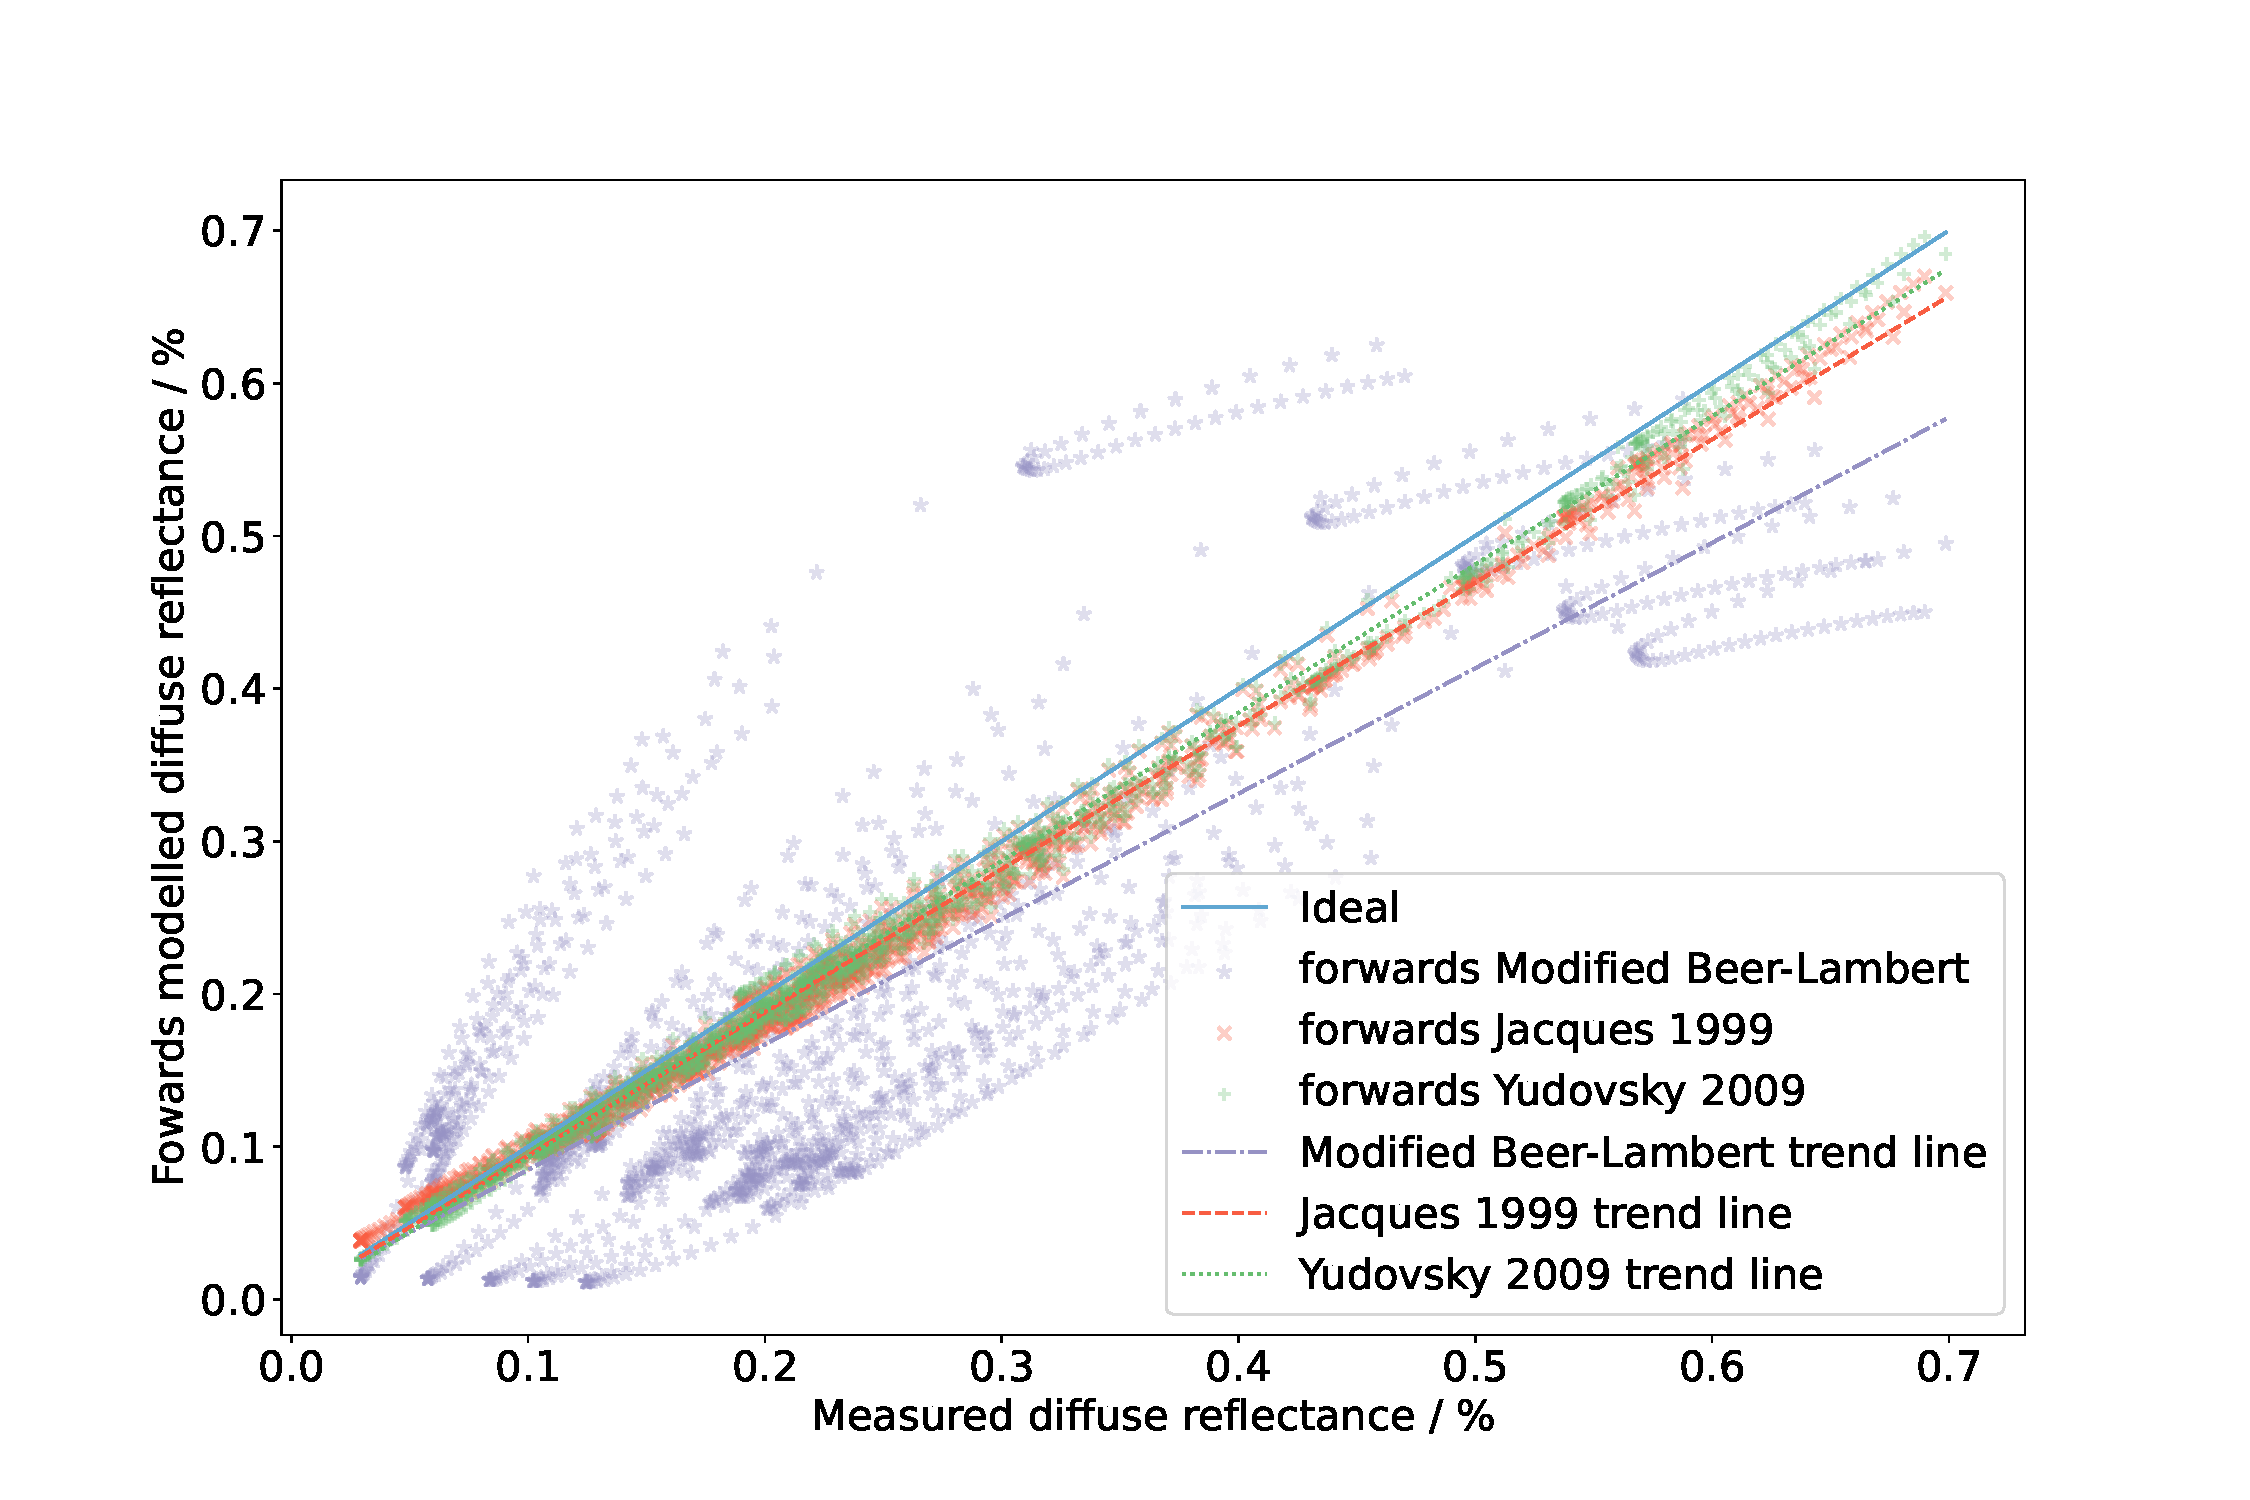
\includegraphics[width=\textwidth]{forwards_v_measured.pdf}
%         \caption{}
%         \label{fig:forwardsregressionphantomquant}
%     \end{subfigure}
%     \begin{subfigure}{0.8\textwidth}
%         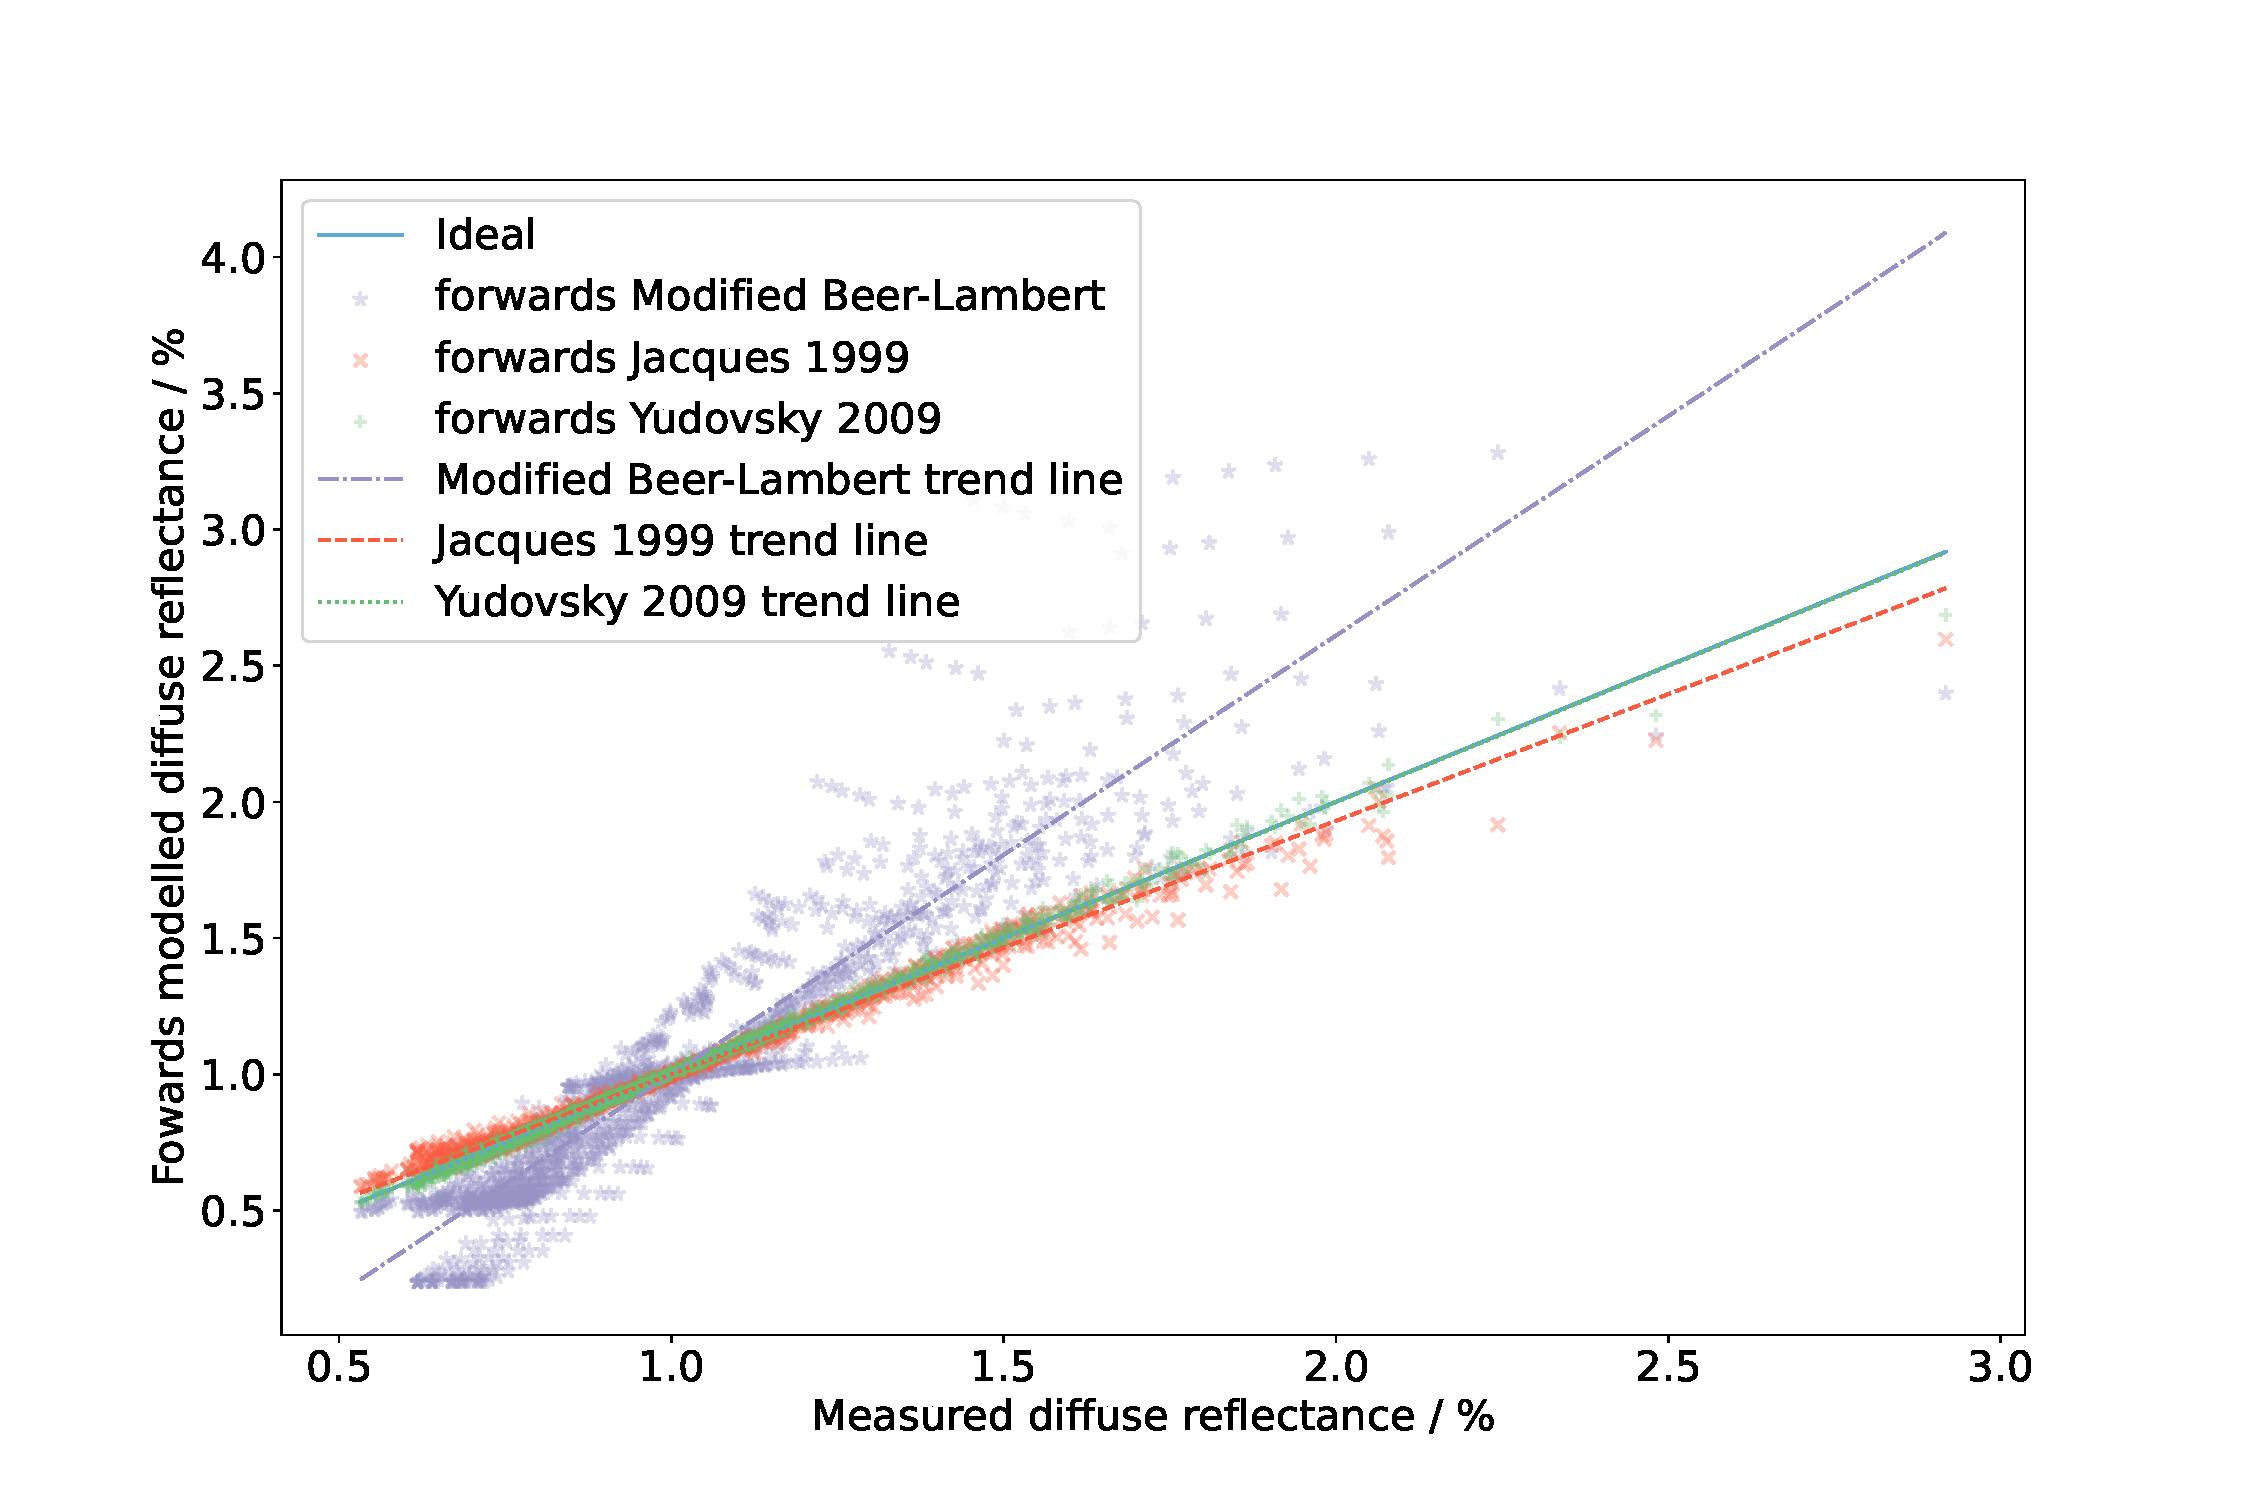
\includegraphics[width=\textwidth]{forwards_v_measured_norm.pdf}
%         \caption{}
%         \label{fig:forwardsregressionphantomnorm}
%     \end{subfigure}
%     \caption{Regression lines between the measured spectra and the analytical models: Yudovsky 2009 (green
%     dotted), Jacques 1999 (red dashed), and Modified Beer-Lambert (orange dot-dashed) for quantitative (\ref{fig:forwardsregressionphantomquant}) or relative (\ref{fig:forwardsregressionphantomnorm}) spectra.}
%  \label{fig:forwardsregressionphantom}
% \end{figure}
% \FloatBarrier

\begin{table}[htb!]
    \centering
    \caption{The regression gradient $m$, offset $c$, Pearson $r$, and $p$ values, and the median (inter-quartile range) absolute percentage errors $APE$ for each variable when extracted by fitting Yudovsky 2009 (Y), Jacques 1999 (J), or Modified Beer-Lambert (BL) to measured tissue phantom spectra for both quantitative and relative data. All presented to 3s.f.}
    \begin{tabular}{|ccc|ccccc|}
        \hline
        Parameter & Model & Quantitative (Q) & $m$ & $c$ & $r$ & $p$ & $APE$ \\
        & & or Relative (R) & (ideal =1) & (ideal = 0) & (ideal = 1) & (ideal = 0) & (\%)\\
        \hline
        \multirow{6}{*}{$AR1$} & \multirow{2}{*}{Y} & Q & 1.00 & 0.0132 & 0.997 & 5.75$\times 10^{-38}$ & 1.59 (11.0) \\
        & & R & 1.01 & -0.0166 & 0.998 & 6.72$\times 10^{-40}$ & 4.42 (8.31) \\
        \cline{2-8}
        & \multirow{2}{*}{J} & Q & 0.976 & 0.0481 & 0.989 & 6.16$\times 10^{-29}$ & 7.02 (20.2) \\
        & & R & 0.905 & 0.0442 & 0.934 & 2.67$\times 10^{-16}$ & 10.4 (23.7) \\
        \cline{2-8}
        & \multirow{2}{*}{BL} & Q & 0.850 & -0.148 & 0.756 & 1.50$\times 10^{-7}$ & 83.5 (57.0) \\
        & & R & 0.730 & -0.107 & 0.939 & 7.84$\times 10^{-17}$ & 50.0 (31.4)\\
        \hline
        \multirow{6}{*}{$AR14$} & \multirow{2}{*}{Y} & Q & 1.00 & -0.0140 & 0.997 & 5.75$\times 10^{-38}$ & 1.36 (8.69) \\
        & & R & 1.01 & 0.00675 & 0.998 & 6.72$\times 10^{-40}$ & 2.48 (5.76) \\
        \cline{2-8}
        & \multirow{2}{*}{J} & Q & 0.976 & -0.0244 & 0.989 & 6.16$\times 10^{-29}$ & 7.02 (16.3) \\
        & & R & 0.905 & 0.0508 & 0.934 & 2.67$\times 10^{-16}$ & 6.34 (10.0) \\
        \cline{2-8}
        & \multirow{2}{*}{BL} & Q & 0.850 & 0.297 & 0.756 & 1.50$\times 10^{-7}$ & 80.4 (72.1) \\
        & & R & 0.730 & 0.377 & 0.939 & 7.84$\times 10^{-17}$ & 37.5 (66.7) \\
        \hline
        \multirow{6}{*}{$I$} & \multirow{2}{*}{Y} & Q & 2.41 & 1.09 & 0.648 & 2.61$\times 10^{-5}$ & 125 (276) \\
        & & R & 0.998 & 1.37 & 0.310 & 6.96$\times 10^{-2}$ & 93.9 (30.0) \\
        \cline{2-8}
        & \multirow{2}{*}{J} & Q & 1.62 & 3.73 & 0.540 & 8.11$\times 10^{-4}$ & 122 (288) \\
        & & R & -0.767 & 4.76 & -0.451 & 6.61$\times 10^{-3}$ & 100 (55.7) \\
        \cline{2-8}
        & \multirow{2}{*}{BL} & Q & -1.75 & 11.8 & -0.705 & 2.29$\times 10^{-6}$ & 100 (172) \\
        & & R & -0.484 & 3.94 & -0.157 & 3.66$\times 10^{-1}$ & 100 (0.00) \\
        \hline
        \multirow{6}{*}{$c_{tot}$} & \multirow{2}{*}{Y} & Q & 1.46 & 9.25 & 0.500 & 2.23$\times 10^{-3}$ & 102 (226) \\
        & & R & 0.917 & 4.85 & 0.303 & 7.72$\times 10^{-2}$ & 66.1 (46.8) \\
        \cline{2-8}
        & \multirow{2}{*}{J} & Q & 2.00 & 6.76 & 0.684 & 5.95$\times 10^{-6}$ & 100 (260) \\
        & & R & -0.265 & 27.8 & -0.0959 & 5.84$\times 10^{-1}$ & 89.7 (267) \\
        \cline{2-8}
        & \multirow{2}{*}{BL} & Q & 0.356 & 3.02 & 0.721 & 1.01$\times 10^{-6}$ & 35.2 (21.6) \\
        & & R & 0.309 & 3.23 & 0.689 & 4.63$\times 10^{-6}$ & 44.6 (23.6) \\
        \hline
    \end{tabular}
    \label{tb:phantomparamsfull}
\end{table}
\FloatBarrier
%
% \section{}\label{ap:3dyefigures}
%
% \FloatBarrier

% \section{}\label{ap:3dyetable}
% \FloatBarrier
% \begin{table}
%     \centering
%     \caption{The  Pearson $r$ (bold if $p<0.05$) of the linear regression line between the fitted tissue parameters and their ground truth displayed with their median (inter-quartile range) absolute percentage errors. This is shown for each variable and for each refractive index dataset when extracted by fitting Yudovsky 2009 (Y), Jacques 1999 (J), or Modified Beer-Lambert (BL) to the Monte-Carlo dataset. All presented to 3s.f.}
% \end{table}

% The mismatch of the forwards model using literature hyperparameters and ground truth tissue parameters to a Monte Carlo simulation of refractive index 1.33 can be seen in an example spectrum in Figure \ref{fig:badJacques}, alongside the improved results from our refitted hyperparameters. 
% \begin{figure}[h!]
%     \centering
%     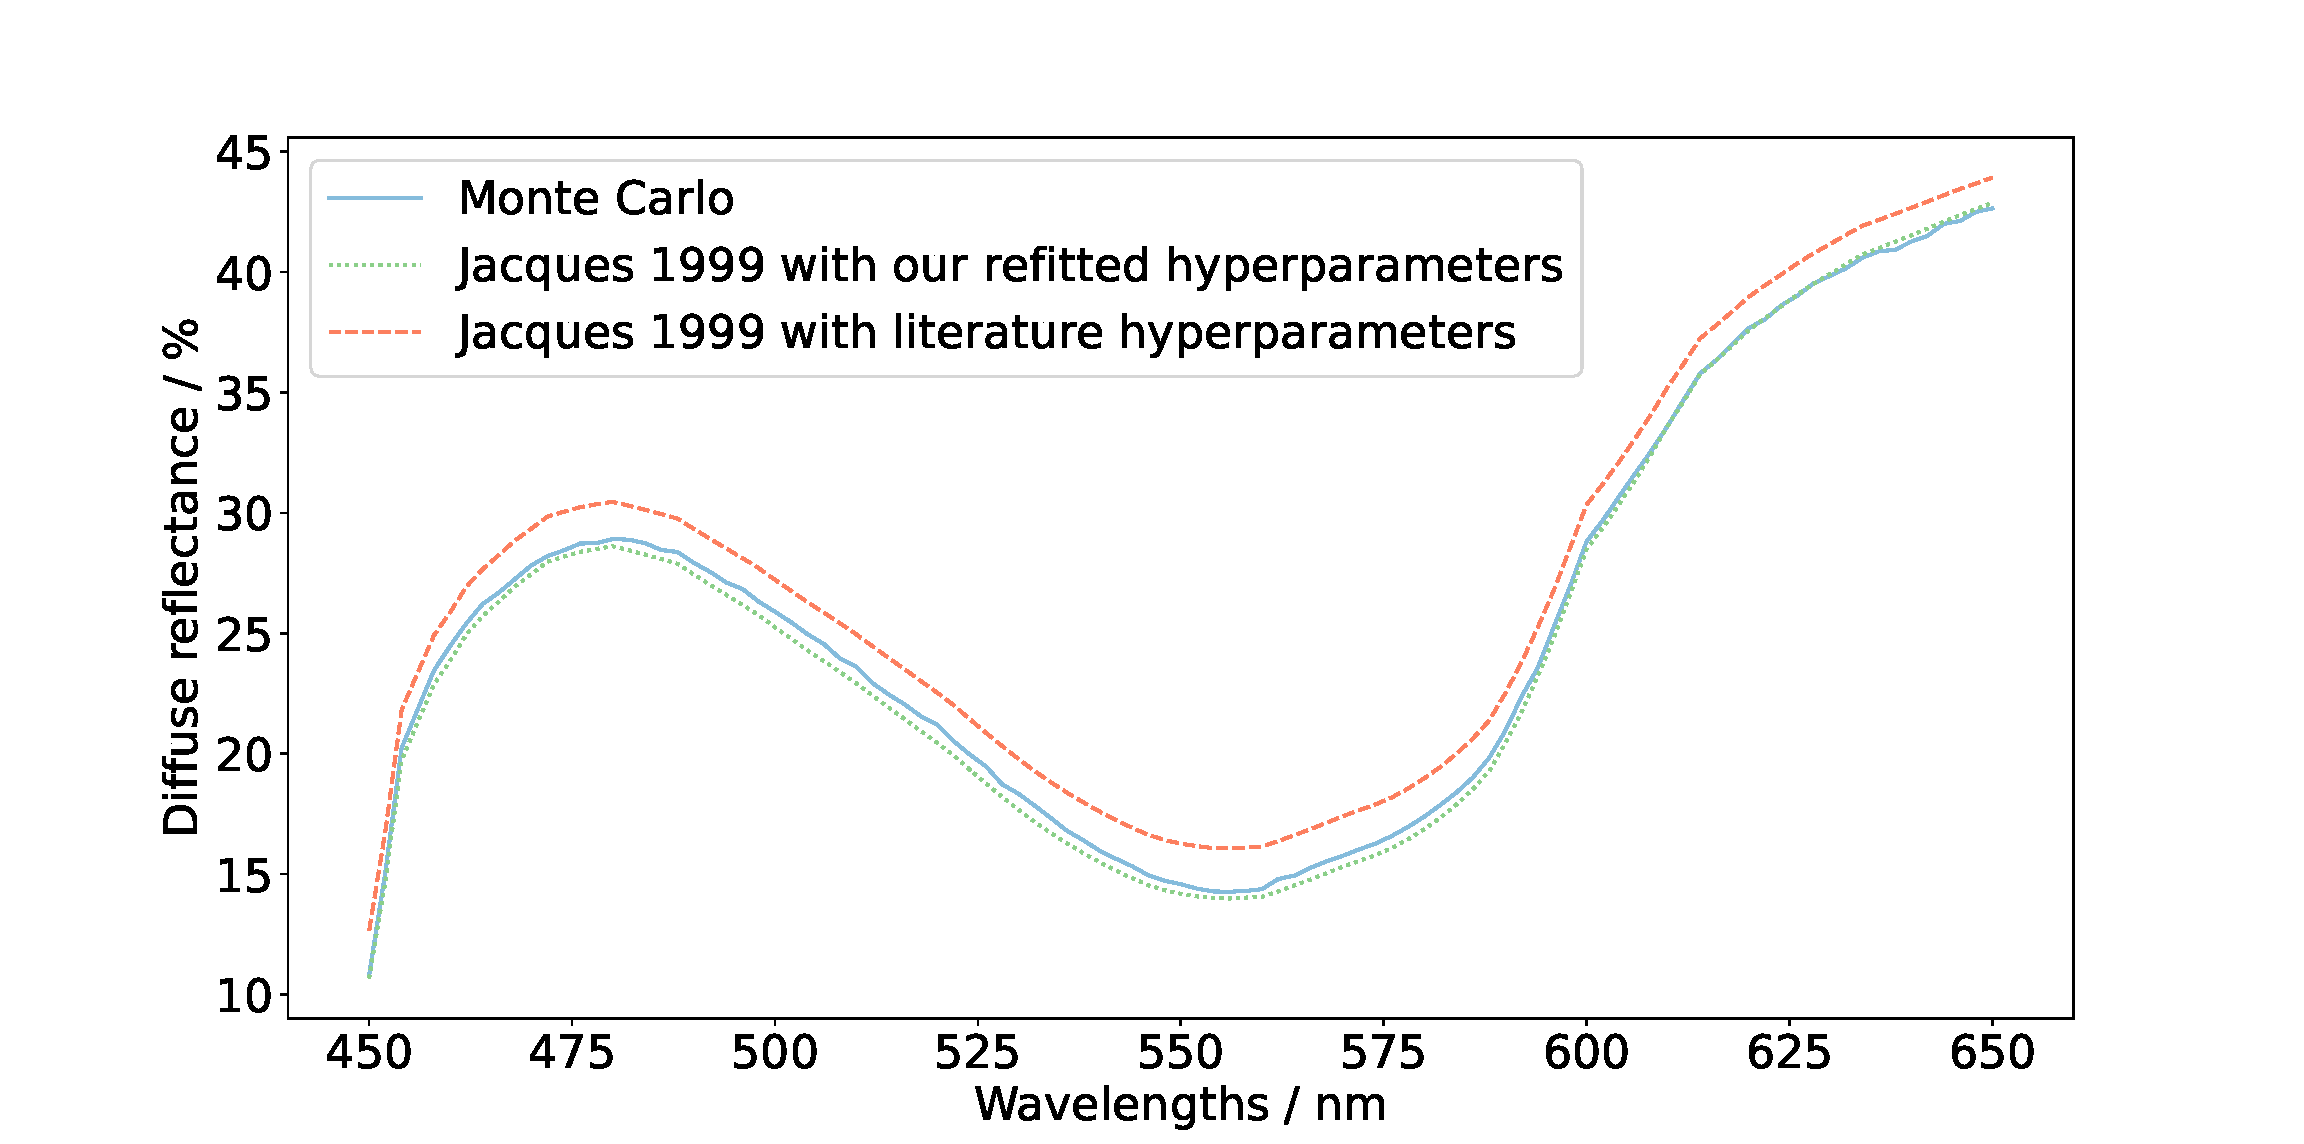
\includegraphics[width=0.65\textwidth]{Jacques_Eg_litvfit}
%     \caption{Example of difference in forwards model similarity to Monte Carlo simulation (blue solid) between modelled spectra using literature Jacques 1999 hyperparameters (red dashed) and our refitted hyperparameters (green dotted) using ground truth variables for a refractive index of 1.33.}
%  \label{fig:badJacques}
% \end{figure}
% 
% \begin{figure}[h!]
%     \centering
%     \begin{subfigure}{0.25\textwidth}
%         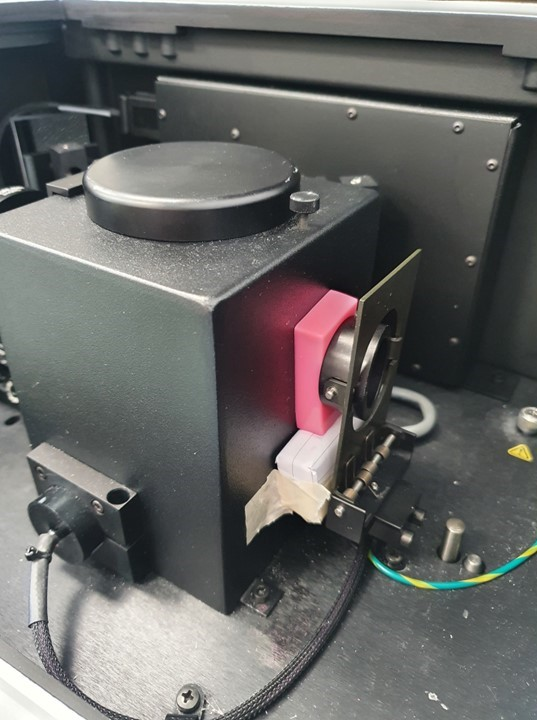
\includegraphics[width=\textwidth]{DiffuseR_img}
%         \caption{}
%         \label{fig:spectrophotometer_dR_img}
%     \end{subfigure}
%     \begin{subfigure}{0.25\textwidth}
%         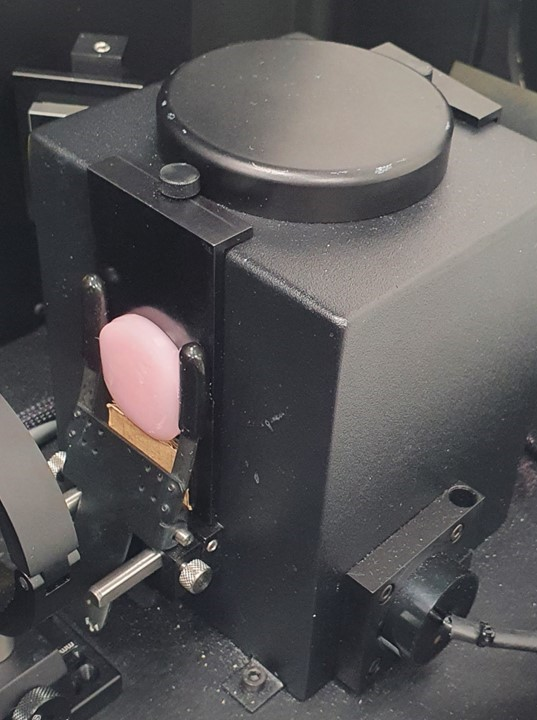
\includegraphics[width=\textwidth]{DiffuseT_img}
%         \caption{}
%         \label{fig:spectrophotometer_dT_img}
%     \end{subfigure}
%     \caption{Images of measurement set-up for diffuse reflectance measurements of 1cm depth gelatin based tissue phantoms (\ref{fig:spectrophotometer_dR_img}) and diffuse transmittance measurements of 5mm depth gelatin based tissue phantoms (\ref{fig:spectrophotometer_dT_img}).}
%     \label{fig:spectrophotometer_img}
% \end{figure}

% \begin{table}
%     \centering
%     \caption{The  Pearson $r$ (bold if $p<0.05$) of the linear regression line between the fitted tissue parameters and their ground truth displayed with their median (inter-quartile range) absolute percentage errors. This is shown for each variable and for each refractive index dataset when extracted by fitting Yudovsky 2009 (Y), Jacques 1999 (J), or Modified Beer-Lambert (BL) to the Monte-Carlo dataset. All presented to 3s.f.}
%     \begin{tabular}{|ccc|cc|}
%         \hline
%         parameter & model & refractive & $r$ & median (inter-quartile range) \\
%         & & index &  & absolute percentage error (\%)\\
%         \hline
%         \multirow{9}{*}{$StO_2$} & \multirow{3}{*}{Y} & 1.33 & \textbf{0.999} & 1.56 (2.56) \\
%         & & 1.35 & \textbf{0.999} & 1.95 (2.88) \\
%         & & 1.44 & \textbf{0.999} & 1.86 (3.32) \\
%         \cline{2-5}
%         & \multirow{3}{*}{J} & 1.33 & \textbf{0.964} & 5.39 (17.1) \\
%         & & 1.35 & \textbf{0.965} & 10.1 (21.2) \\
%         & & 1.44 & \textbf{0.963} & 5.22 (19.9) \\
%         \cline{2-5}
%         & \multirow{3}{*}{BL} & 1.33 & \textbf{0.648} & 52.4 (76.5) \\
%         & & 1.35 & \textbf{0.694} & 71.3 (57.6) \\
%         & & 1.44 & \textbf{0.735} & 54.2 (70.8) \\
%         \hline
%         \multirow{9}{*}{$f_{blood}$} & \multirow{3}{*}{Y} & 1.33 & \textbf{0.992} & 4.38 (6.30) \\
%         & & 1.35 & \textbf{0.985} & 4.13 (6.86) \\
%         & & 1.44 & \textbf{0.984} & 4.36 (5.98) \\
%         \cline{2-5}
%         & \multirow{3}{*}{J} & 1.33 & \textbf{0.947} & 9.79 (8.55) \\
%         & & 1.35 & \textbf{0.924} & 9.63 (11.68) \\
%         & & 1.44 & \textbf{0.930} & 8.04 (9.10) \\
%         \cline{2-5}
%         & \multirow{3}{*}{BL} & 1.33 & \textbf{0.745} & 28.2 (32.6) \\
%         & & 1.35 & \textbf{0.505} & 54.1 (31.0) \\
%         & & 1.44 & \textbf{0.710} & 27.8 (29.3) \\
%         \hline
%         \multirow{9}{*}{$a$} & \multirow{3}{*}{Y} & 1.33 & \textbf{0.996} & 4.61 (5.03) \\
%         & & 1.35 & \textbf{0.995} & 4.79 (5.23) \\
%         & & 1.44 & \textbf{0.992} & 3.46 (4.45) \\
%         \cline{2-5}
%         & \multirow{3}{*}{J} & 1.33 & \textbf{0.974} & 6.70 (7.15) \\
%         & & 1.35 & \textbf{0.965} & 7.32 (11.3) \\
%         & & 1.44 & \textbf{0.970} & 4.51 (8.94) \\
%         \cline{2-5}
%         & \multirow{3}{*}{BL} & 1.33 & \textbf{-0.686} & 88.0 (132) \\
%         & & 1.35 & \textbf{-0.455} & 96.4 (180) \\
%         & & 1.44 & \textbf{-0.747} & 86.6 (131) \\
%         \hline
%         \multirow{9}{*}{$b$} & \multirow{3}{*}{Y} & 1.33 & \textbf{0.994} & 2.08 (4.32) \\
%         & & 1.35 & \textbf{0.994} & 3.78 (7.52) \\
%         & & 1.44 & \textbf{0.997} & 3.24 (5.14) \\
%         \cline{2-5}
%         & \multirow{3}{*}{J} & 1.33 & \textbf{0.918} & 14.3 (33.9) \\
%         & & 1.35 & \textbf{0.948} & 18.7 (36.0) \\
%         & & 1.44 & \textbf{0.928} & 11.8 (31.6) \\
%         \cline{2-5}
%         & \multirow{3}{*}{BL} & 1.33 & \textbf{-0.345} & 96.0 (54.2) \\
%         & & 1.35 & \textbf{-0.354} & 94.6 (11.6) \\
%         & & 1.44 & \textbf{-0.341} & 94.3 (97.6) \\
%         \hline
%     \end{tabular}
%     \label{tb:singleparamtrends}
% \end{table}
\section{Investigating two layer model using uniform wavelength weighting}\label{ap:2layeruniform}
This section presents a similar inverse problem fitting analysis to the results presented in Chapter \ref{chap:2layer}, however the wavelength weighting used here is uniform. There are limited changes to the conclusions so further discussion is not provided, however it should be noted that the visual fitting of the 525-585nm of the NIST spectra is worsened using this configuration.

\subsection{Simulated data}
\begin{figure}[htbp]
    \centering
    \begin{subfigure}{0.49\textwidth}
        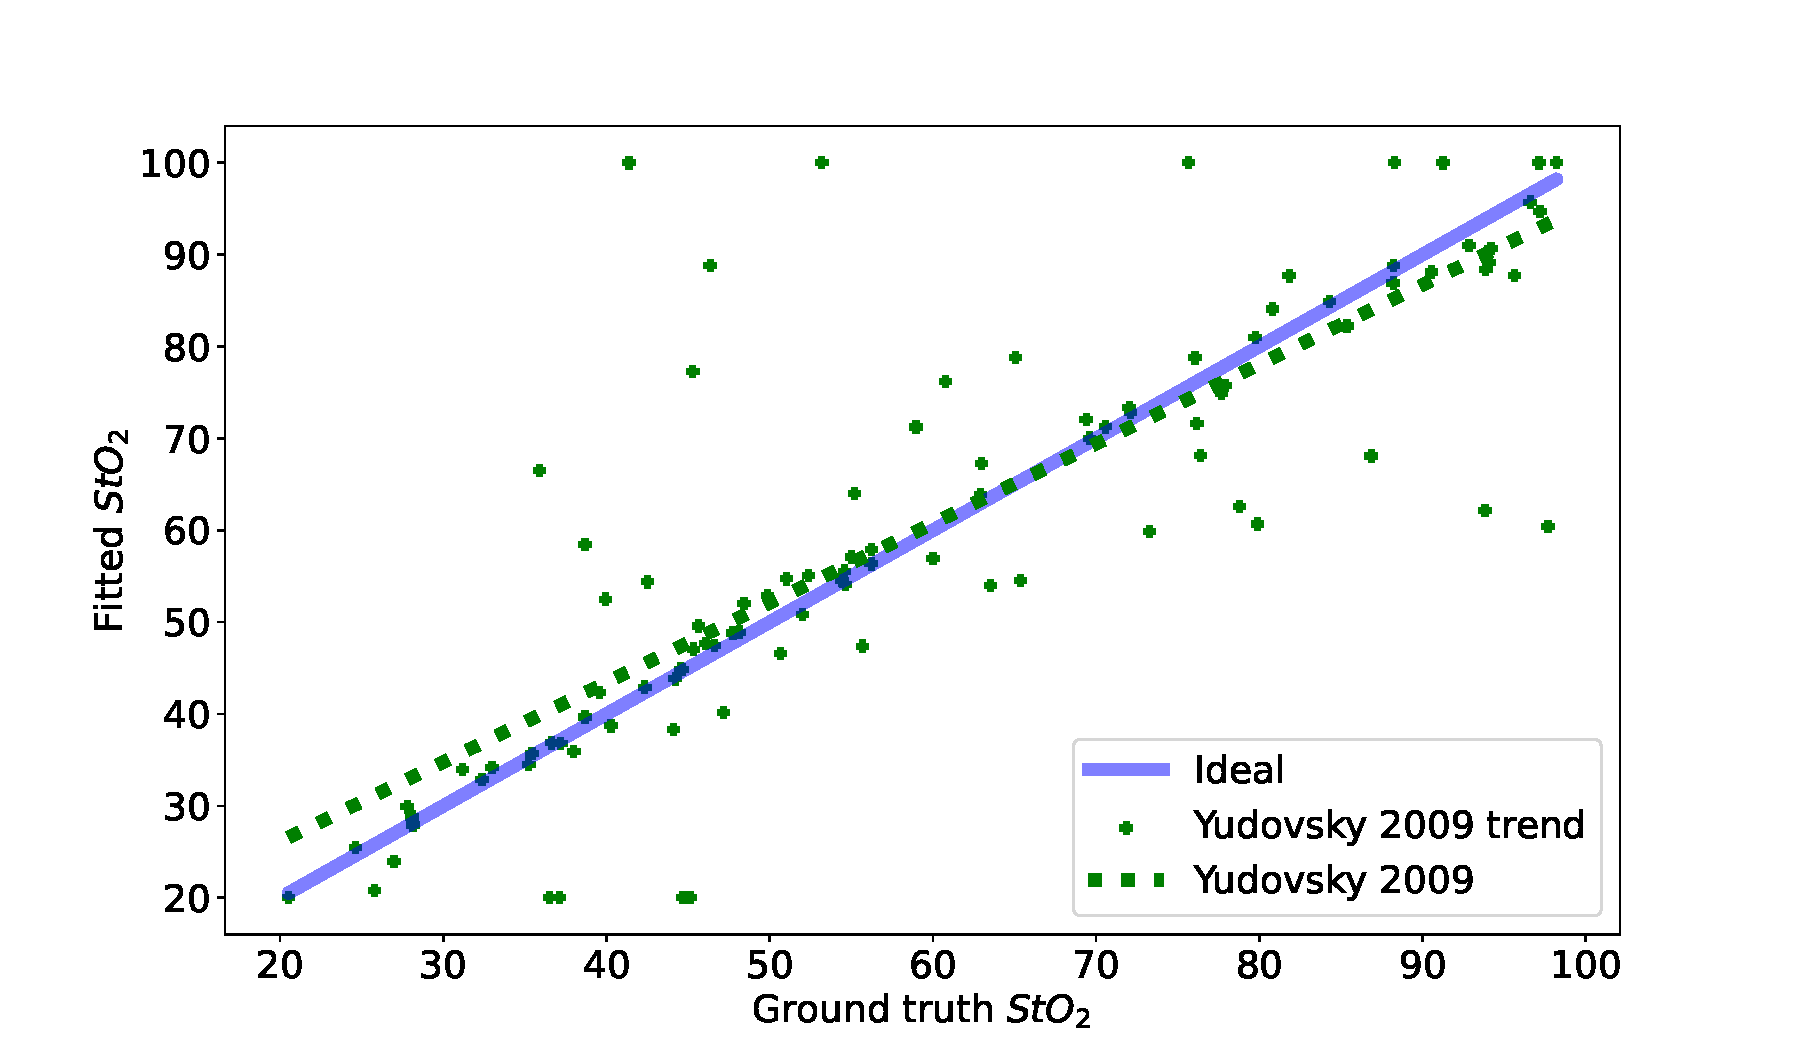
\includegraphics[width=\textwidth]{StO2_twolayer_MC_uniform.pdf}
        \caption{Quantitative}
        \label{fig:egparamsStO2MCu}
    \end{subfigure}
    \begin{subfigure}{0.49\textwidth}
        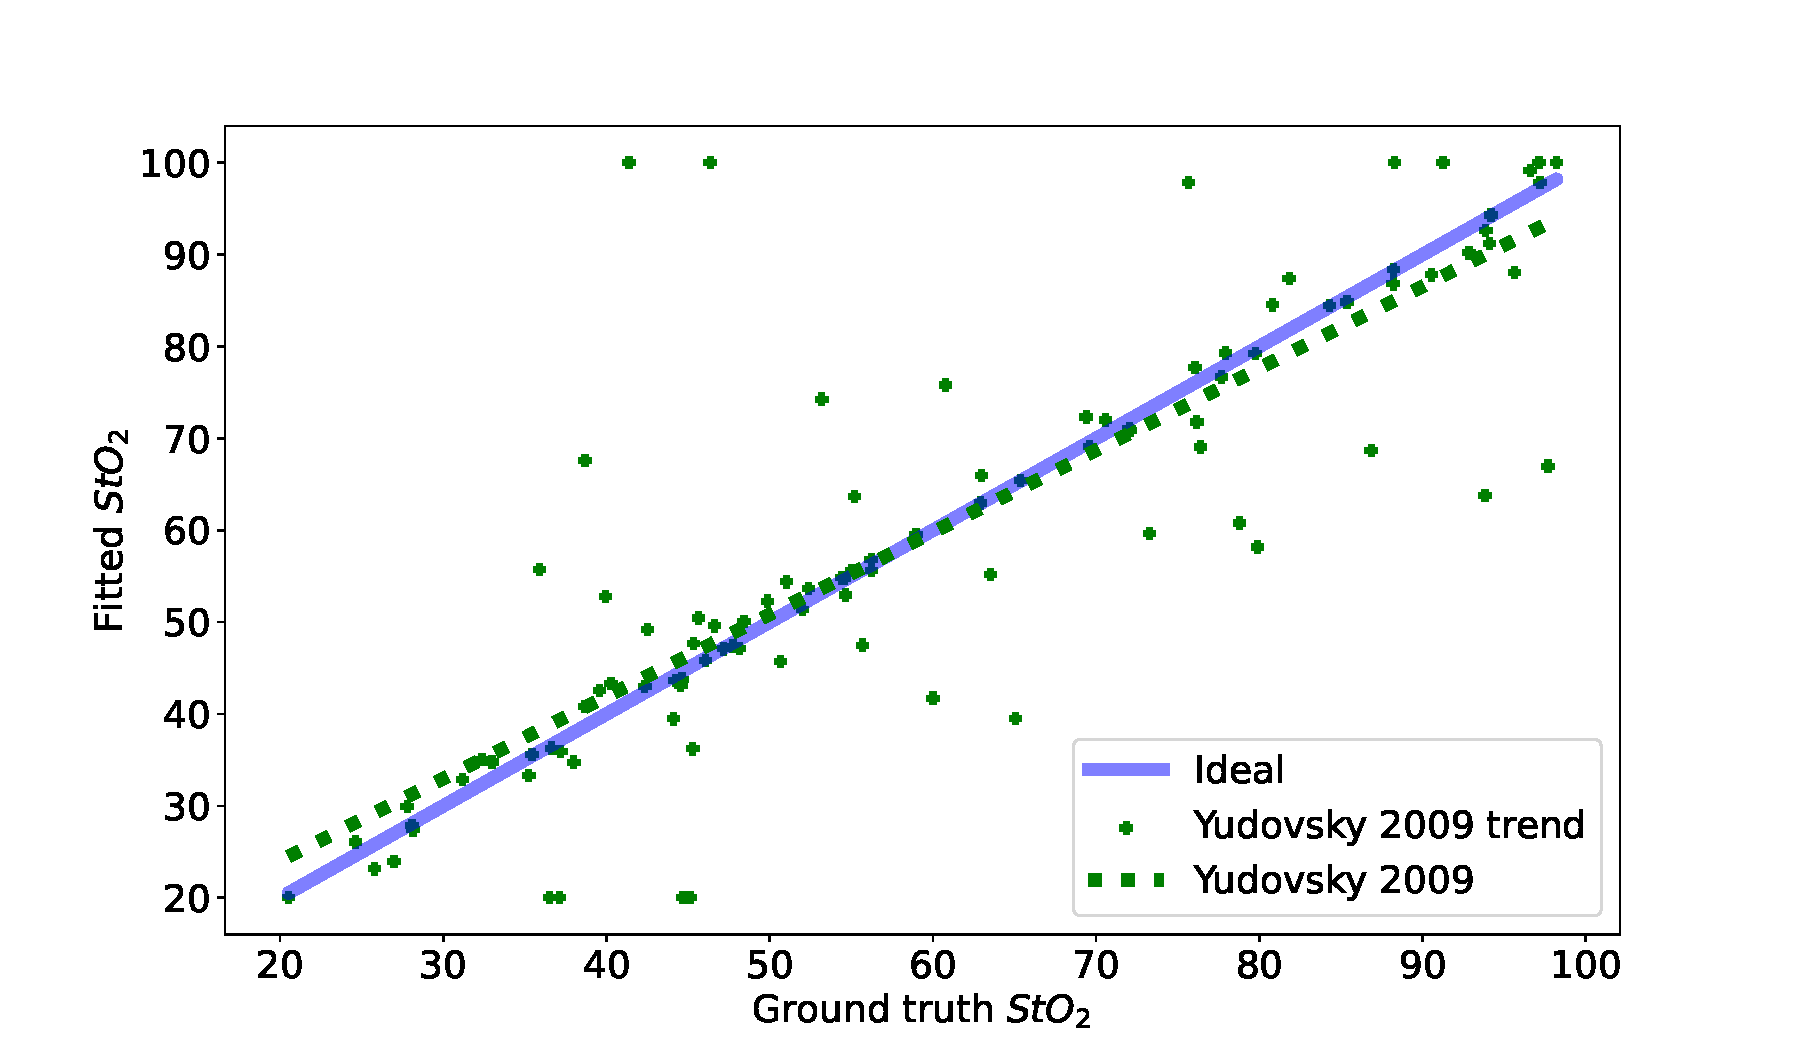
\includegraphics[width=\textwidth]{StO2_twolayer_MC_norm_uniform.pdf}
        \caption{Relative}
        \label{fig:egparamsStO2MCnormu}
    \end{subfigure}
    \begin{subfigure}{0.49\textwidth}
        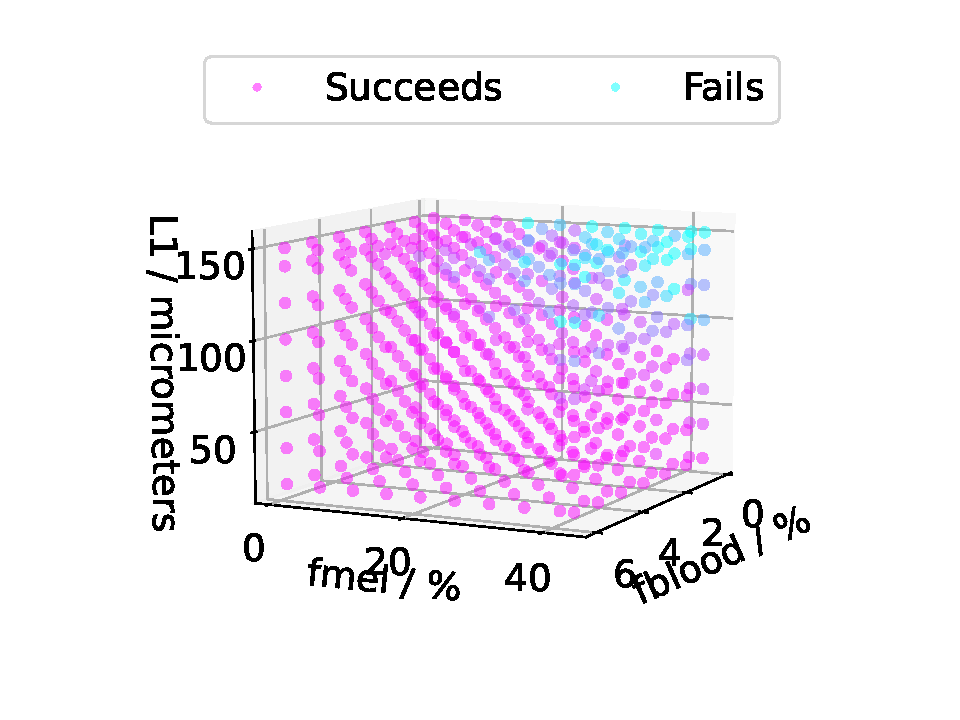
\includegraphics[width=\textwidth]{2layer_parameter_exploration_uniform.pdf}
        \caption{Quantitative}
        \label{fig:egparamsfailureMCu}
    \end{subfigure}
    \begin{subfigure}{0.49\textwidth}
        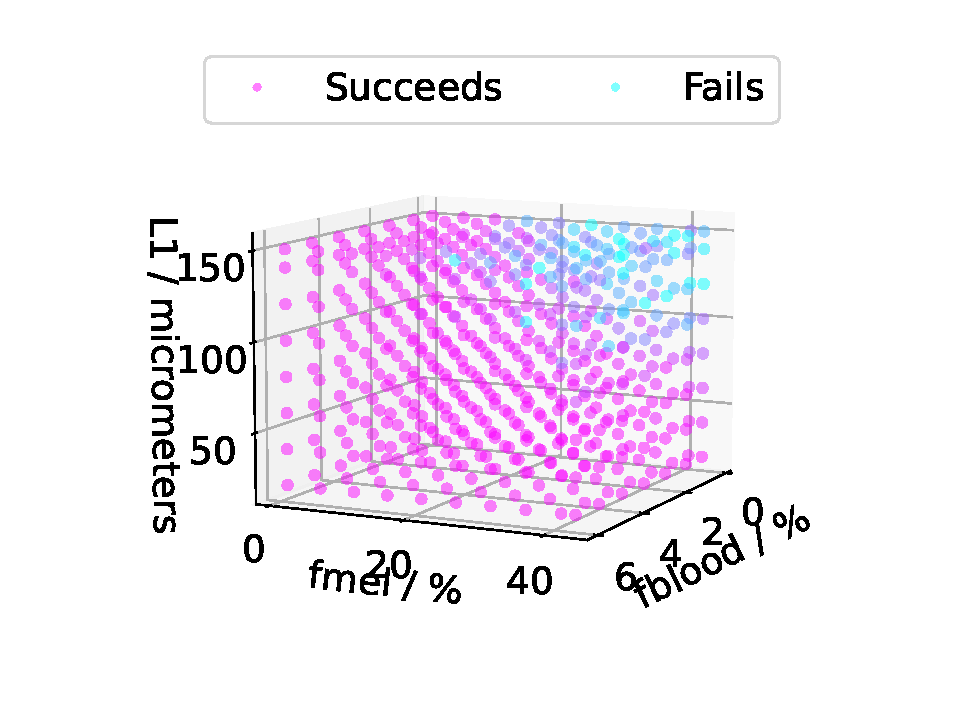
\includegraphics[width=\textwidth]{2layer_parameter_norm_uniform.pdf}
        \caption{Relative}
        \label{fig:egparamsfailureMCnormu}
    \end{subfigure}
    \caption{Top: Example $StO_2$ recovery from fitting Yudovsky 2009 two layer model to Monte Carlo simulated diffuse reflectance and the associated linear regression line between the extracted and ground truth parameters for quantitative (left) or relative (right) data. Bottom: a depiction of the impact of 3 key physiological parameters on success of $StO_2$ extraction by visualising the Pearson $r$ correlation coefficient for the extracted $StO_2$ compared to the ground-truth for simulations with this range of parameters extracted using Yudovsky 2009 two-layer model for quantitative (left) or relative (right) data.}
    \label{fig:MC2layeruniform}
\end{figure}

\begin{table}[h]
    \centering
    \caption{The regression gradient $m$, offset $c$, Pearson $r$ (bold if $p<0.05$), and the mean ($\pm$ standard deviation) absolute percentage errors for each variable when extracted by fitting Yudovsky 2009 two layer model to the quantitative or relative Monte-Carlo diffuse reflectance dataset with uniform weighting of wavelengths. All presented to 3s.f.}
    \begin{tabular}{|c|c|cccc|}
        \hline
        parameter & Quantitative & $m$ & $c$ & $r$ & mean ($\pm$ standard deviation) \\
        & or Relative & (ideal =1) & (ideal = 0) & (ideal = 1) & absolute percentage error (\%)\\
        \hline
        \multirow{2}{*}{$StO_2$} & Quantitative & 0.866 & 8.81 & \textbf{0.821} & 14.2($\pm$ 23.1) \\
        & Relative & 0.893 & 6.18 & \textbf{0.842} & 13.0($\pm$ 22.2) \\
        \hline
        \multirow{2}{*}{$f_{blood}$} & Quantitative & 0.956 & 0.160 & \textbf{0.856} & 25.1($\pm$ 25.3) \\
        & Relative & 0.839 & 3.35$\times 10^{-2}$ & \textbf{0.706} & 30.9($\pm$ 25.9) \\
        \hline
        \multirow{2}{*}{$f_{mel}$} & Quantitative & 0.838 & 1.17 & \textbf{0.875} & 23.9($\pm$ 18.6) \\
        & Relative & 0.497 & 5.45 & \textbf{0.531} & 35.4($\pm$ 25.0) \\
        \hline
        \multirow{2}{*}{$L_1$} & Quantitative & 0.840 & 31.3 & \textbf{0.824} & 37.1($\pm$ 39.1) \\
         & Relative & 0.827 & 34.9 & \textbf{0.805} & 39.0($\pm$ 36.6) \\
        \hline
        \multirow{2}{*}{$a$} & Quantitative & 0.682 & 13.3 & \textbf{0.586} & 19.4($\pm$ 14.6) \\
        & Relative & 0.515 & 20.5 & \textbf{0.389} & 26.1($\pm$ 22.3) \\
        \hline
        \multirow{2}{*}{$b$} & Quantitative & 0.804 & 0.338 & \textbf{0.781} & 14.2($\pm$ 16.4) \\
        & Relative & 0.729 & 0.521 & \textbf{0.586} & 25.1($\pm$ 26.7) \\
        \hline
    \end{tabular}
    \label{tb:doubleparamtrendsuniform}
\end{table}
\FloatBarrier

\subsection{NIST}
\begin{figure}[h]
    \centering
    \begin{subfigure}{0.49\textwidth}
        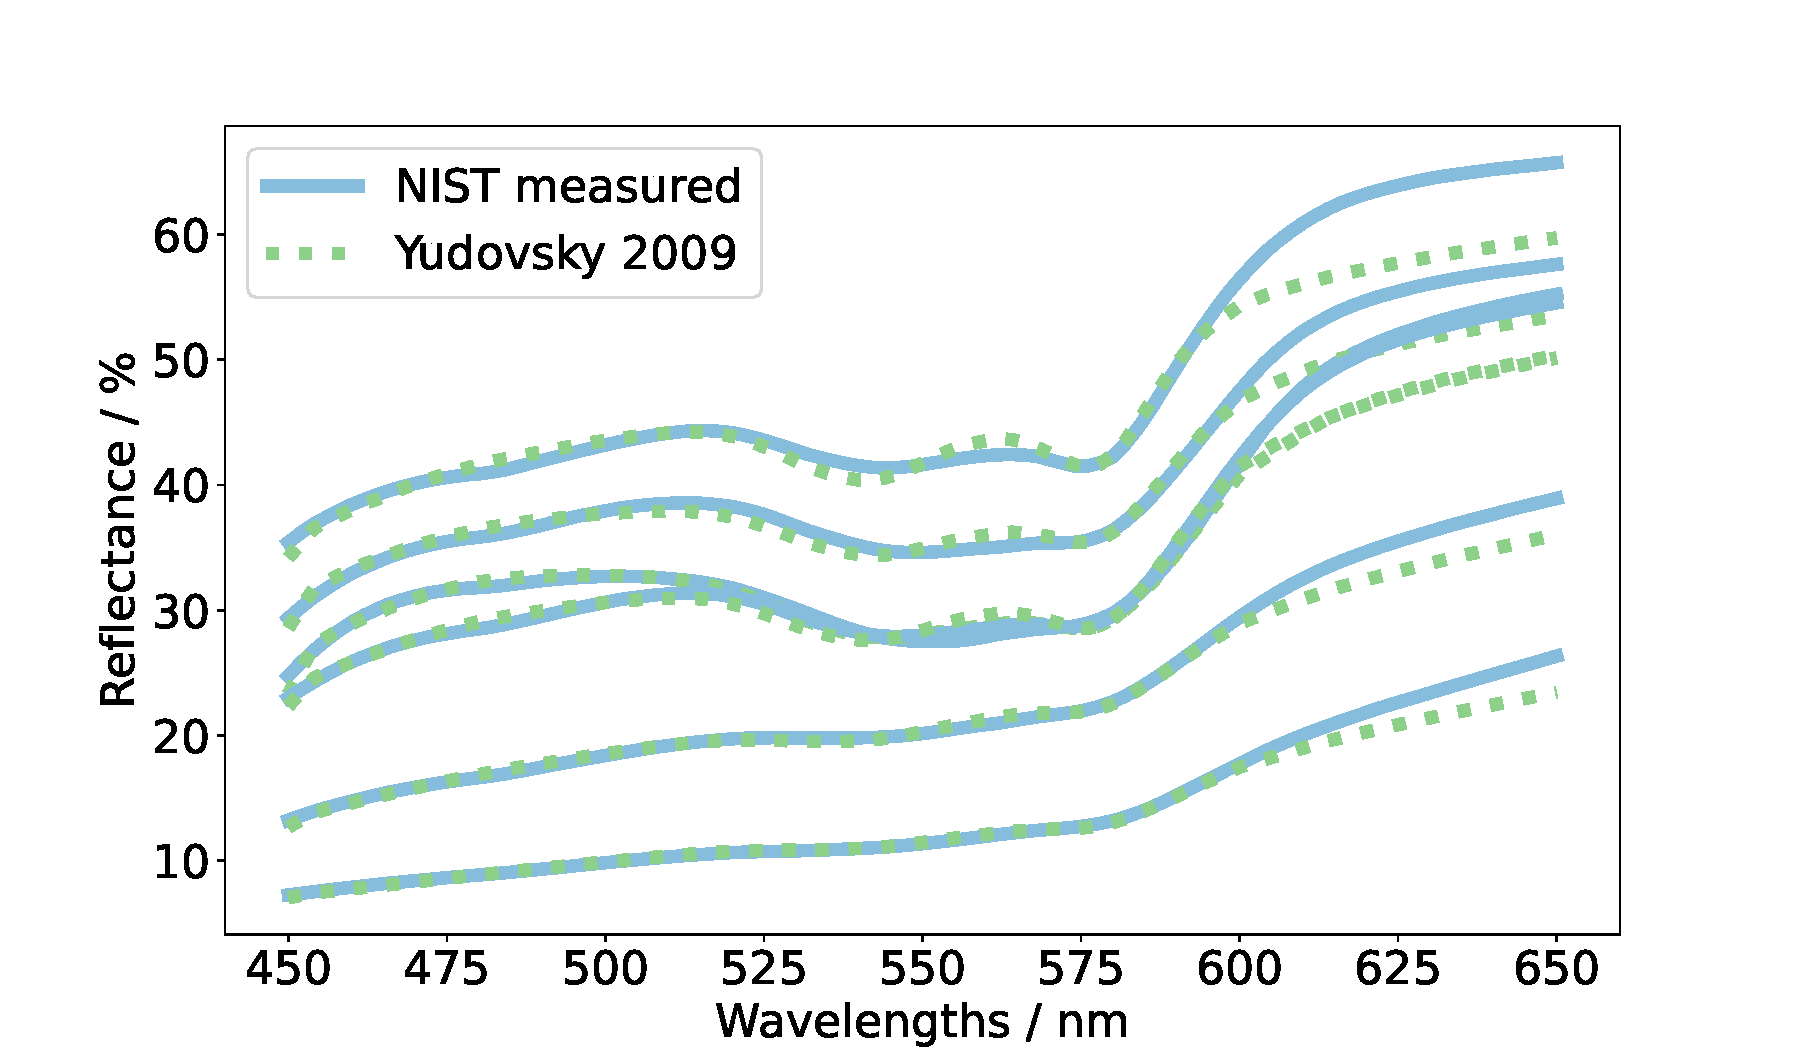
\includegraphics[width=\textwidth]{NIST_Eg_uniform.pdf}
        \caption{Quantitative}
        \label{fig:egspectraNISTu}
    \end{subfigure}
    \begin{subfigure}{0.49\textwidth}
        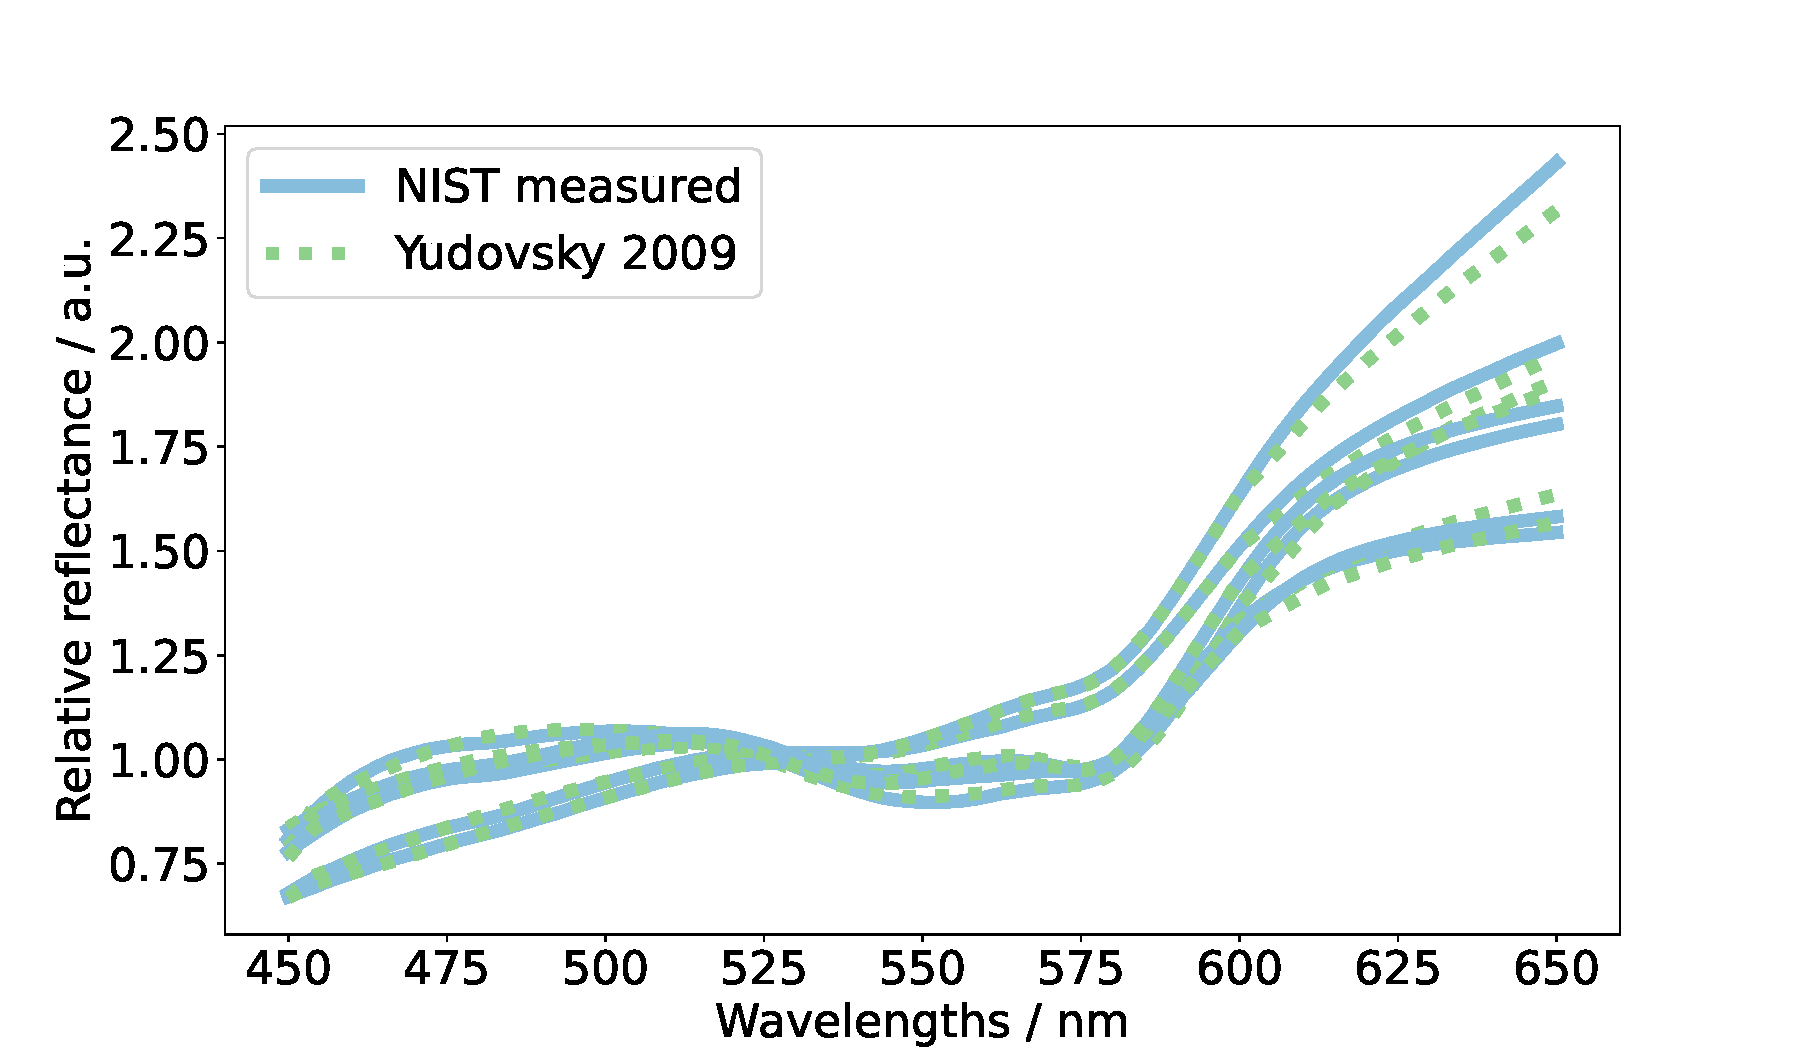
\includegraphics[width=\textwidth]{NIST_Eg_norm_uniform.pdf}
        \caption{Relative}
        \label{fig:egspectraNISTnormu}
    \end{subfigure}
    \begin{subfigure}{0.49\textwidth}
        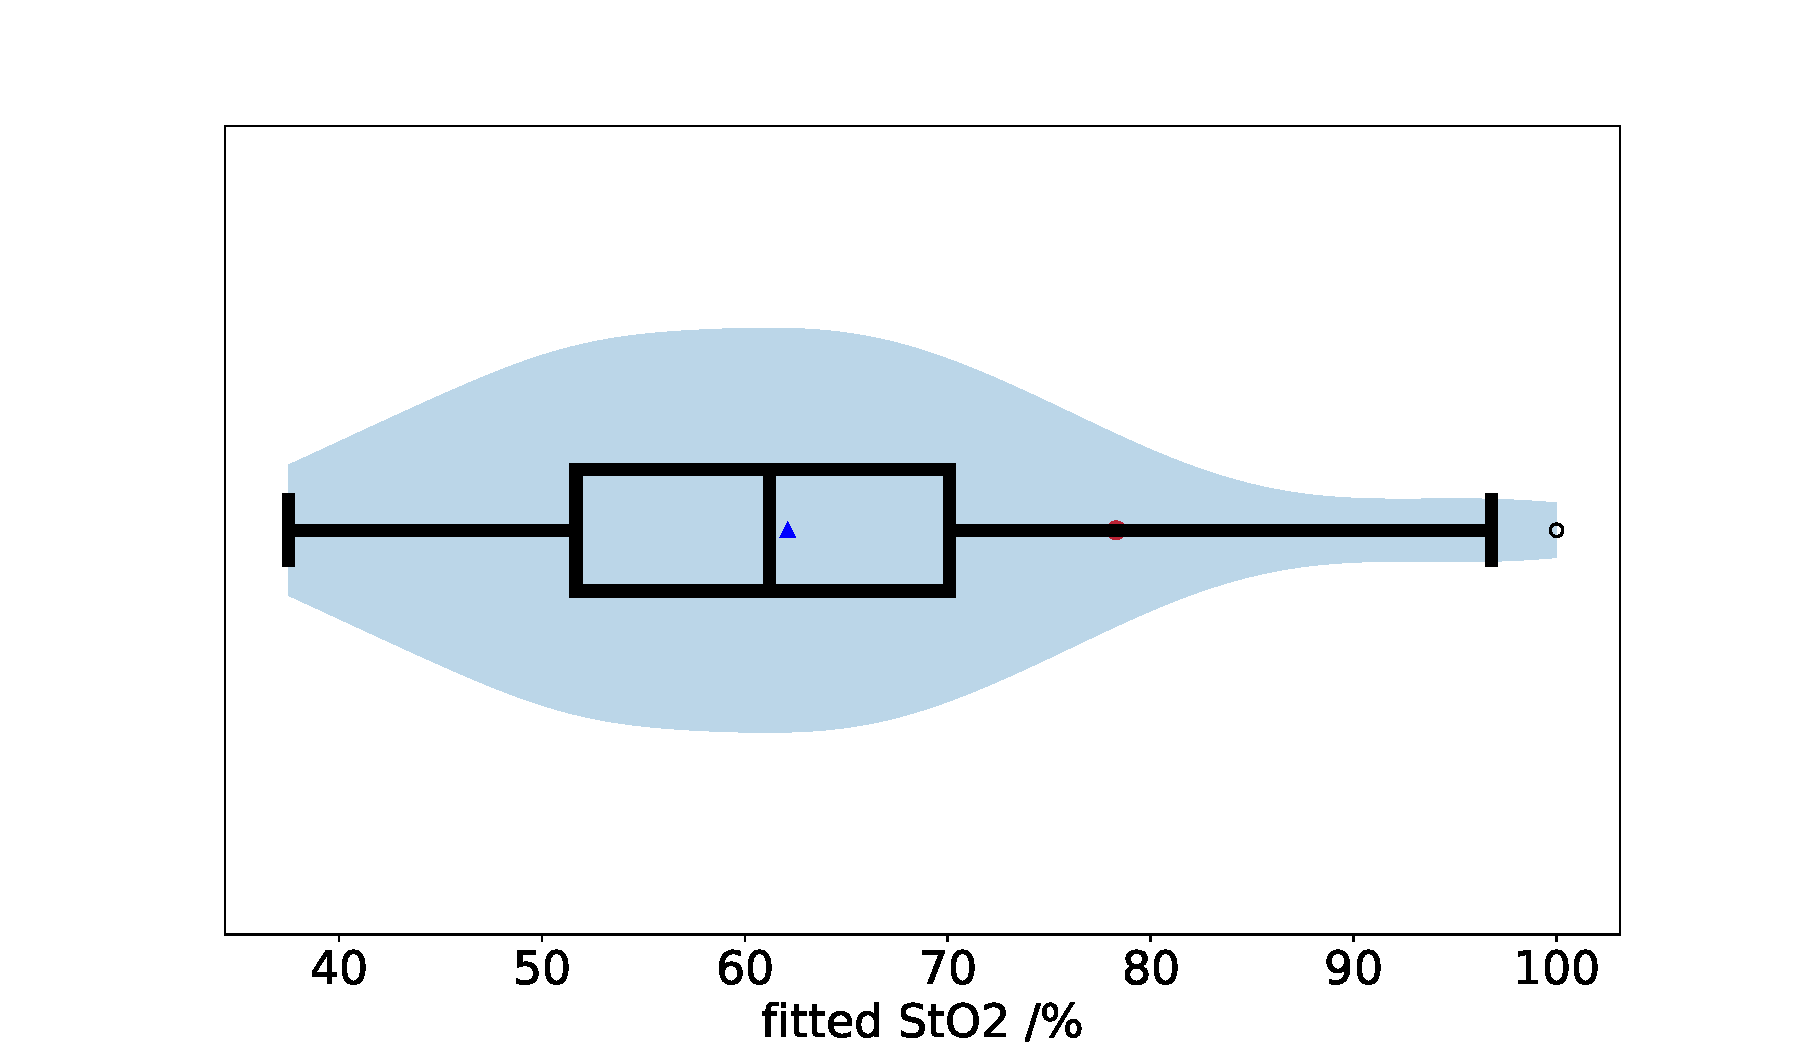
\includegraphics[width=\textwidth]{StO2_boxplot_uniform.pdf}
        \caption{Quantitative}
        \label{fig:egparamStO2NISTu}
    \end{subfigure}
    \begin{subfigure}{0.49\textwidth}
        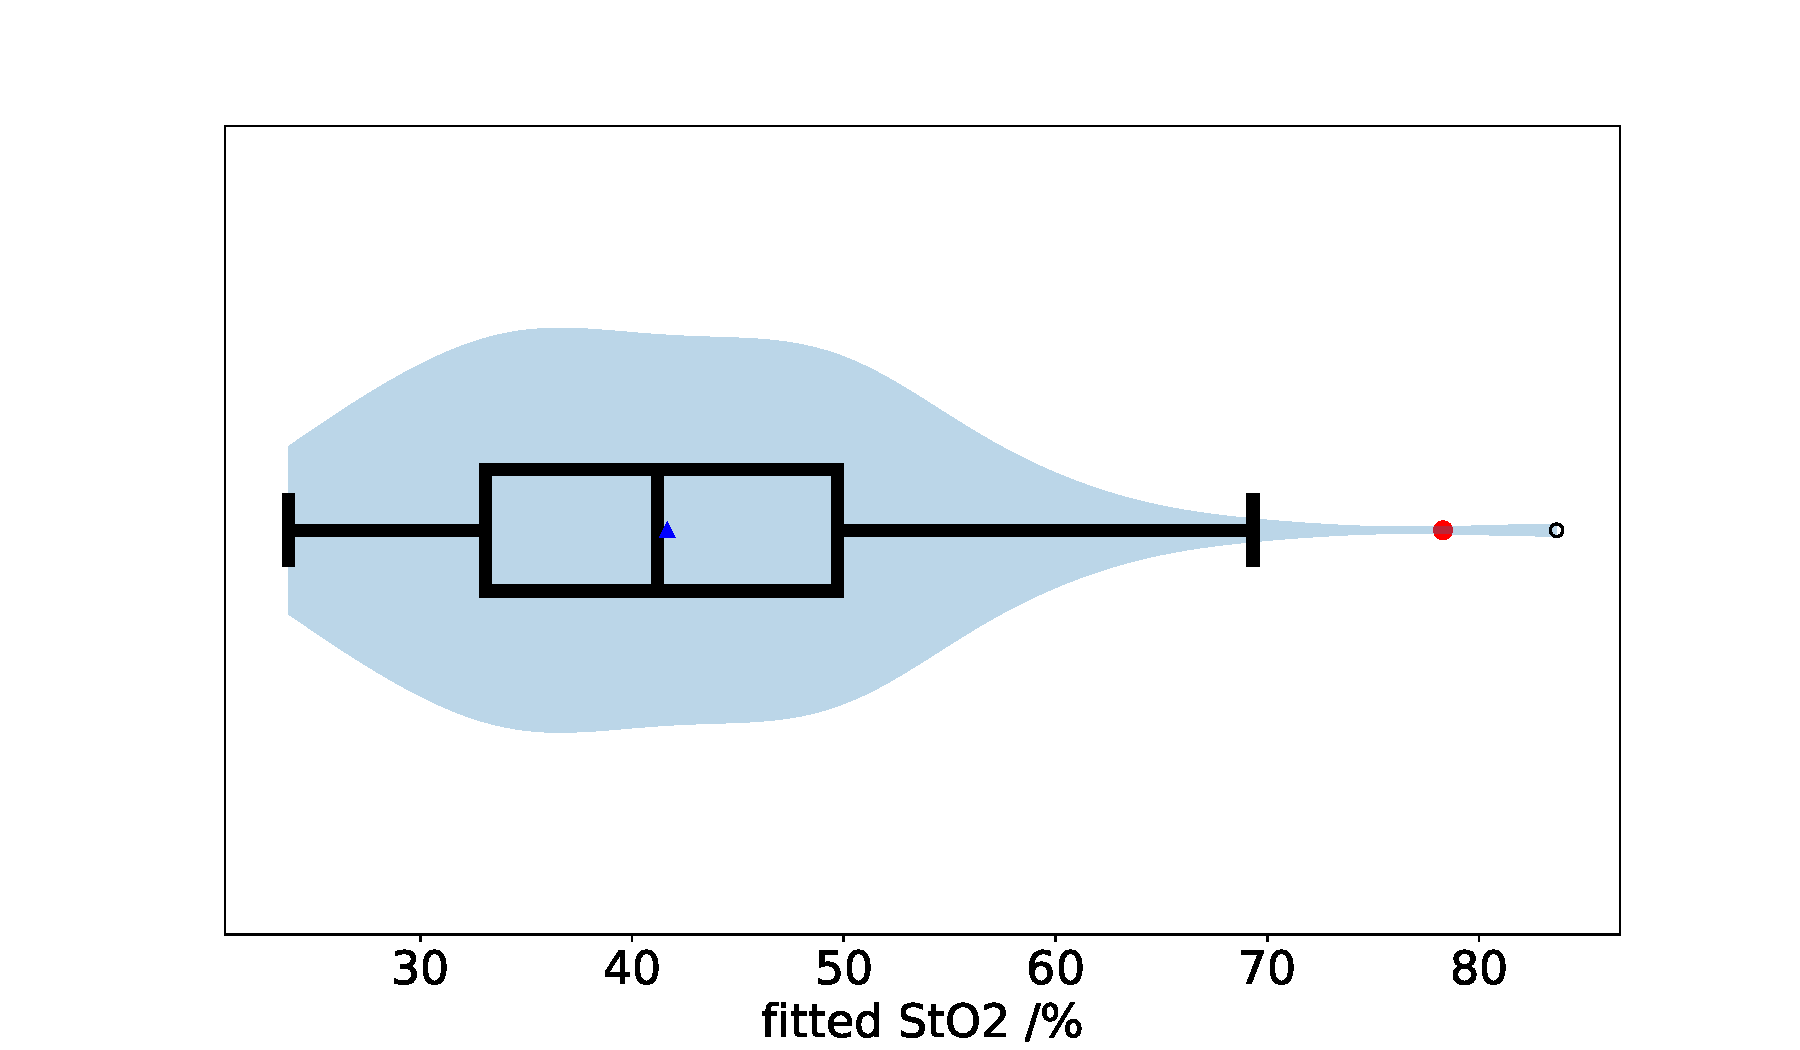
\includegraphics[width=\textwidth]{StO2_boxplot_norm_uniform.pdf}
        \caption{Relative}
        \label{fig:egparamStO2NISTnormu}
    \end{subfigure}
    \caption{Top: Examples of the Yudovsky 2009 two layer model fitted to NIST skin total reflectance spectra (\figref{fig:egspectraNIST}) for quantitative (left) or relative (right) data. Bottom: Box and violin plots displaying the retrieved $StO_2$ parameters from fitting the Yudovsky 2009 two layer model to the mean NIST skin spectra, where the triangle shows the mean of the fitted $StO_2$ and the circle shows a literature healthy dermis $StO_2$ value \cite{VanManen2021} for quantitative (left) or relative (right) data.}
    \label{fig:NISTuniform}
\end{figure}
\begin{table}[h]
    \centering
    \caption{The mean and standard deviation for each variable when extracted by fitting Yudovsky 2009 two layer model to the quantitative or relative NIST skin reflectance dataset, compared to literature parameters for healthy individuals. All presented to 3s.f.}
    \begin{tabular}{|c|ccc|ccc|}
        \hline
        \multirow{2}{*}{Parameter} & \multicolumn{3}{c}{Extracted from NIST dataset} & \multicolumn{3}{|c|}{Literature} \\
        \cline{2-7}
         & Quantitative & \multirow{2}{*}{Mean} & Standard & \multirow{2}{*}{Mean} & Standard & \multirow{2}{*}{Source} \\
         & or Relative &  & deviation &  & deviation &  \\
        \hline
        \multirow{2}{*}{$StO_2$ (\%)} & Quantitative & 62.1 & 14.5 & \multirow{2}{*}{78.3, 71} & \multirow{2}{*}{12.9, 16} & \multirow{2}{*}{\cite{VanManen2021}, \cite{Nishidate2011}} \\ %van manen http://dx.doi.org/10.21037/qims-21-46
        & Relative & 41.7 & 11.0 & & & \\ %Noninvasive imaging of human skin hemodynamicsusing a digital red-green-blue camera
        \hline
        $f_{blood}$ (\%) & Quantitative & 0.875 & 0.443 & \multirow{2}{*}{1.1} & \multirow{2}{*}{0.4} & \multirow{2}{*}{\cite{Nishidate2011}} \\ %Noninvasive imaging of human skin hemodynamicsusing a digital red-green-blue camera
        & Relative & 1.66 & 0.996 & & & \\
        \hline
        $f_{mel}$ (\%) & Quantitative & 2.57 & 3.95 & \multirow{2}{*}{4.3} & \multirow{2}{*}{1.2} & \multirow{2}{*}{\cite{Nishidate2011}} \\ %Noninvasive imaging of human skin hemodynamicsusing a digital red-green-blue camera
        & Relative & 3.03 & 2.18 & & &  \\
        \hline
        $L_1$ ($\mu$m) & Quantitative & 66.2 & 20.5 & \multirow{2}{*}{75.5} & \multirow{2}{*}{N/A} & \multirow{2}{*}{\cite{Lintzeri2022}} \\ %https://www.webofscience.com/wos/woscc/full-record/WOS:000782026000001
        & Relative & 147 & 8.74 & & &  \\
        \hline
        $a$ (\textrm{$cm^{-1}$}) & Quantitative & 70.0 & 2.29$\times 10^{-8}$ & \multirow{2}{*}{46.0} & \multirow{2}{*}{13.7} & \multirow{2}{*}{\cite{Jacques2013}} \\ %Jacques review
        & Relative & 45.7 & 11.4 & & &  \\
        \hline
        $b$ (a.u.) & Quantitative & 1.01 & 0.382 & \multirow{2}{*}{1.421} & \multirow{2}{*}{0.517} & \multirow{2}{*}{\cite{Jacques2013}} \\ %Jacques review
        & Relative & 2.46 & 0.221 & & &  \\
        \hline
    \end{tabular}
    \label{tb:NISTparamsuniform}
\end{table}

\section{Investigating simulated HSI camera data}
\begin{table}[bhp]
    \centering
    \caption{Mean ($\pm$ standard deviation) $NRMSE$ (3.d.p.) between the simulated camera responses of each forwards spectrum from each model and each of 100 Monte Carlo simulated spectra using the same ground truth variable parameters for each refractive index dataset for quantitative data at a variety of noise levels (0, 1\%, 3\%). This is presented with the Pearson $r$ (bold if Pearson $p < 0.05$) for the linear regression between all forwards spectra against Monte Carlo simulated spectra for each refractive index dataset and each analytical model. All metrics are evaluated for the wavelength region of 450-600nm.}
    \begin{tabular}{|cc|c|ccc|ccc|}
        \hline
        Model & Layers & Refractive & \multicolumn{3}{|c}{$NRMSE$} & \multicolumn{3}{|c|}{$r$} \\
         & & index & 0 & 1\% & 3\% & 0 & 1\% & 3\% \\
        \hline
        \multirow{3}{*}{\shortstack{Yudovsky\\ 2009}} & \multirow{3}{*}{1} & 1.33 & \shortstack{0.012 \\($\pm$ 0.006)} & \shortstack{0.077 \\($\pm$ 0.054)} & \shortstack{0.204 \\($\pm$ 0.128)} & \textbf{1.000} & \textbf{0.996} & \textbf{0.959} \\
        & & 1.35 & \shortstack{0.011 \\($\pm$ 0.005)} & \shortstack{0.088 \\($\pm$ 0.063)} & \shortstack{0.241 \\($\pm$ 0.150)} & \textbf{1.000} & \textbf{0.993} & \textbf{0.944} \\
        & & 1.44 & \shortstack{0.009 \\($\pm$ 0.004)} & \shortstack{0.082 \\($\pm$ 0.057)} & \shortstack{0.224 \\($\pm$ 0.125)} & \textbf{1.000} & \textbf{0.993} & \textbf{0.942} \\
        \hline
        \multirow{3}{*}{\shortstack{Jacques\\ 1999}} & \multirow{3}{*}{1} & 1.33 & \shortstack{0.033 \\($\pm$ 0.063)} & \shortstack{0.086 \\($\pm$ 0.084)} & \shortstack{0.206 \\($\pm$ 0.137)} & \textbf{1.000} & \textbf{0.995} & \textbf{0.959} \\
        & & 1.35 & \shortstack{0.040 \\($\pm$ 0.071)} & \shortstack{0.100 \\($\pm$ 0.092)} & \shortstack{0.242 \\($\pm$ 0.153)} & \textbf{0.999} & \textbf{0.992} & \textbf{0.943} \\
        & & 1.44 & \shortstack{0.026 \\($\pm$ 0.046)} & \shortstack{0.089 \\($\pm$ 0.077)} & \shortstack{0.227 \\($\pm$ 0.130)} & \textbf{1.000} & \textbf{0.993} & \textbf{0.942} \\
        \hline
        \shortstack{Yudovsky\\ 2009} & 2 & 1.44 & \shortstack{0.166 \\($\pm$ 0.133)} & \shortstack{0.482 \\($\pm$ 0.289)} & \shortstack{0.738 \\($\pm$ 0.294)} & \textbf{0.992} & \textbf{0.971} & \textbf{0.829} \\
        \hline
    \end{tabular}
    \label{ap:forwardsHSIMCq}
\end{table}
\FloatBarrier

\begin{table}[bhp]
    \centering
    \caption{Mean ($\pm$ standard deviation) $NRMSE$ (3.d.p.) between the simulated camera responses of each forwards spectrum from each model and each of 100 Monte Carlo simulated spectra using the same ground truth variable parameters for each refractive index dataset for relative data at a variety of noise levels (0, 1\%, 3\%). This is presented with the Pearson $r$ (bold if Pearson $p < 0.05$) for the linear regression between all forwards spectra against Monte Carlo simulated spectra for each refractive index dataset and each analytical model. All metrics are evaluated for the wavelength region of 450-600nm.}
    \begin{tabular}{|cc|c|ccc|ccc|}
        \hline
        Model & Layers & Refractive & \multicolumn{3}{|c}{$NRMSE$} & \multicolumn{3}{|c|}{$r$} \\
         & & index & 0 & 1\% & 3\% & 0 & 1\% & 3\% \\
        \hline
        \multirow{3}{*}{\shortstack{Yudovsky\\ 2009}} & \multirow{3}{*}{1} & 1.33 & \shortstack{0.004 \\($\pm$ 0.003)} & \shortstack{0.071 \\($\pm$ 0.057)} & \shortstack{0.203 \\($\pm$ 0.142)} & \textbf{1.000} & \textbf{0.908} & \textbf{0.559} \\
        & & 1.35 & \shortstack{0.003 \\($\pm$ 0.003)} & \shortstack{0.085 \\($\pm$ 0.063)} & \shortstack{0.237 \\($\pm$ 0.150)} & \textbf{1.000} & \textbf{0.886} & \textbf{0.530} \\
        & & 1.44 & \shortstack{0.003 \\($\pm$ 0.002)} & \shortstack{0.075 \\($\pm$ 0.044)} & \shortstack{0.212 \\($\pm$ 0.118)} & \textbf{1.000} & \textbf{0.916} & \textbf{0.602} \\
        \hline
        \multirow{3}{*}{\shortstack{Jacques\\ 1999}} & \multirow{3}{*}{1} & 1.33 & \shortstack{0.018 \\($\pm$ 0.026)} & \shortstack{0.073 \\($\pm$ 0.062)} & \shortstack{0.204 \\($\pm$ 0.144)} & \textbf{0.992} & \textbf{0.899} & \textbf{0.545} \\
        & & 1.35 & \shortstack{0.021 \\($\pm$ 0.029)} & \shortstack{0.087 \\($\pm$ 0.064)} & \shortstack{0.239 \\($\pm$ 0.152)} & \textbf{0.990} & \textbf{0.884} & \textbf{0.519} \\
        & & 1.44 & \shortstack{0.014 \\($\pm$ 0.021)} & \shortstack{0.076 \\($\pm$ 0.045)} & \shortstack{0.212 \\($\pm$ 0.117)} & \textbf{0.995} & \textbf{0.915} & \textbf{0.605} \\
        \hline
        \shortstack{Yudovsky\\ 2009} & 2 & 1.44 & \shortstack{0.033 \\($\pm$ 0.026)} & \shortstack{0.428 \\($\pm$ 0.286)} & \shortstack{0.684 \\($\pm$ 0.286)} & \textbf{0.991} & \textbf{0.270} & -0.007 \\
        \hline
    \end{tabular}
    \label{ap:forwardsHSIMCr}
\end{table}
\FloatBarrier

\begin{table}[htb!]
    \centering
    \caption{The Pearson $r$ values (bold if $p<0.05$) of the linear regression line between the fitted tissue parameters and their ground truth displayed with their median (inter-quartile range) absolute percentage errors. This is shown for each variable and for each refractive index dataset when extracted by fitting Yudovsky 2009 single layer (Y1), Jacques 1999 (J), or Yudovsky 2009 double layer (Y2) to the quantitative Monte-Carlo datasets at each noise level (0, 1\%, 3\%). All presented to 3s.f.}
    \begin{tabular}{|ccc|ccc|ccc|}
        \hline
        Parameter & Model & Refractive & \multicolumn{3}{c}{$r$} & \multicolumn{3}{|c|}{median (inter-quartile range)} \\
        & & index & \multicolumn{3}{c}{} & \multicolumn{3}{|c|}{absolute percentage error (\%)} \\
        & & & 0 & 1\% & 3\% & 0 & 1\% & 3\% \\
        \hline
        \multirow{7}{*}{$StO_2$} & \multirow{3}{*}{Y1} & 1.33 & \textbf{0.999} & \textbf{0.794} & \textbf{0.403} & 2.25 (5.70) & 40.2 (74.5) & 79.5 (75.6) \\
        & & 1.35 & \textbf{0.999} & \textbf{0.668} & \textbf{0.628} & 1.41 (3.91) & 29.4 (27.4) & 54.4 (79.3) \\
        & & 1.44 & \textbf{0.999} & \textbf{0.825} & \textbf{0.369} & 1.90 (2.83) & 24.8 (60.7) & 85.2 (69.9) \\
        \cline{2-9}
        & \multirow{3}{*}{J} & 1.33 & \textbf{0.967} & \textbf{0.797} & \textbf{0.435} & 5.28 (19.1) & 30.7 (59.3) & 83.1 (71.2) \\
        & & 1.35 & \textbf{0.962} & \textbf{0.807} & \textbf{0.629} & 4.57 (24.0) & 31.2 (64.4) & 51.4 (81.4) \\
        & & 1.44 &  \textbf{0.978} & \textbf{0.829} & \textbf{0.402} & 4.06 (11.3) & 22.5 (60.8) & 83.6 (77.7) \\
        \cline{2-9}
        & Y2 & 1.44 & \textbf{0.751} & 0.0612 & 0.0194 & 16.8 (25.5) & 66.5 (51.5) & 68.9 (55.3) \\
        \hline
        \multirow{7}{*}{$f_{blood}$} & \multirow{3}{*}{Y1} & 1.33 & \textbf{0.980} & \textbf{0.743} & \textbf{0.552} & 2.25 (5.70) & 27.1 (33.7) & 45.7 (43.5) \\
        & & 1.35 & \textbf{0.974} & \textbf{0.668} & \textbf{0.386} & 4.26 (7.53) & 29.4 (27.4) & 51.6 (52.5) \\
        & & 1.44 & \textbf{0.984} & \textbf{0.667} & \textbf{0.450} & 5.83 (6.97) & 23.7 (38.9) & 51.8 (44.3)\\
        \cline{2-9}
        & \multirow{3}{*}{J} & 1.33 & \textbf{0.918} & \textbf{0.768} & \textbf{0.604} & 8.68 (23.6) & 26.6 (35.3) & 42.6 (49.4) \\
        & & 1.35 & \textbf{0.912} & \textbf{0.736} & \textbf{0.432} & 11.3 (18.8) & 27.7 (34.8) & 48.2 (45.9) \\
        & & 1.44 & \textbf{0.924} & \textbf{0.719} & \textbf{0.498} & 7.14 (15.9) & 25.0 (39.4) & 46.7 (42.4) \\
        \cline{2-9}
        & Y2 & 1.44 & \textbf{0.872} & 0.147 & 0.0329 & 23.1 (25.4) & 115 (197) & 160 (291) \\
        \hline
        \multirow{7}{*}{$a$} & \multirow{3}{*}{Y1} & 1.33 & \textbf{0.993} & \textbf{0.828} & \textbf{0.677} & 5.34 (6.11) & 19.1 (25.1) & 29.0 (40.5) \\
        & & 1.35 & \textbf{0.995} & \textbf{0.824} & \textbf{0.627} & 3.61 (5.95) & 20.0 (25.5) & 36.7 (39.7) \\
        & & 1.44 & \textbf{0.992} & \textbf{0.773} & \textbf{0.558} & 3.85 (5.16) & 18.7 (34.7) & 35.1 (39.1) \\
        \cline{2-9}
        & \multirow{3}{*}{J} & 1.33 & \textbf{0.955} & \textbf{0.817} & \textbf{0.682} & 6.33 (20.5) & 19.5 (25.3) & 25.9 (37.6) \\
        & & 1.35 & \textbf{0.968} & \textbf{0.815} & \textbf{0.641} & 8.47 (17.0) & 20.0 (26.4) & 37.1 (38.6) \\
        & & 1.44 & \textbf{0.961} & \textbf{0.759} & \textbf{0.542} & 4.69 (14.0) & 17.1 (31.8) & 30.4 (39.9) \\
        \cline{2-9}
        & Y2 & 1.44 & \textbf{0.674} & 0.00365 & 0.0666 & 17.9 (13.8) & 37.8 (26.8) & 37.4 (26.1) \\
        \hline
        \multirow{9}{*}{$b$} & \multirow{3}{*}{Y1} & 1.33 & \textbf{0.996} & \textbf{0.689} & \textbf{0.370} & 2.28 (3.17) & 25.4 (54.9) & 55.5 (72.2) \\
        & & 1.35 & \textbf{0.996} & \textbf{0.682} & \textbf{0.426} & 2.24 (3.94) & 36.0 (75.1) & 58.2 (69.6) \\
        & & 1.44 & \textbf{0.998} & \textbf{0.751} & \textbf{0.516} & 2.63 (3.63) & 21.8 (46.8) & 52.0 (68.3) \\
        \cline{2-9}
        & \multirow{3}{*}{J} & 1.33 & \textbf{0.874} & \textbf{0.679} & \textbf{0.410} & 5.13 (12.8) & 30.0 (54.0) & 58.0 (74.6) \\
        & & 1.35 & \textbf{0.838} & \textbf{0.646} & \textbf{0.446} & 6.22 (34.2) & 40.4 (74.2) & 57.8 (71.4) \\
        & & 1.44 & \textbf{0.934} & \textbf{0.757} & \textbf{0.515} & 5.70 (16.5) & 23.7 (52.9) & 50.4 (71.4) \\
        \cline{2-9}
        & Y2 & 1.44 & \textbf{0.735} & 0.169 & -0.00249 & 16.8 (19.3) & 56.4 (48.2) & 61.3 (54.9) \\
        \hline
        $f_mel$ & Y2 & 1.44 & \textbf{0.852} & \textbf{0.622} & \textbf{0.477} & 28.0 (31.7) & 85.1 (128) & 90.1 (120) \\
        \hline
        $L_1$ & Y2 & 1.44 & \textbf{0.824} & \textbf{0.401} & 0.123 & 36.7 (40.9) & 69.5 (83.1) & 84.5 (96.0) \\
        \hline
    \end{tabular}    
    \label{ap:backwardsHSIMCq}
\end{table}

\begin{table}[htb!]
    \centering
    \caption{The Pearson $r$ values (bold if $p<0.05$) of the linear regression line between the fitted tissue parameters and their ground truth displayed with their median (inter-quartile range) absolute percentage errors. This is shown for each variable and for each refractive index dataset when extracted by fitting Yudovsky 2009 single layer (Y1), Jacques 1999 (J), or Yudovsky 2009 double layer (Y2) to the relative Monte-Carlo datasets at each noise level (0, 1\%, 3\%). All presented to 3s.f.}
    \begin{tabular}{|ccc|ccc|ccc|}
        \hline
        Parameter & Model & Refractive & \multicolumn{3}{c}{$r$} & \multicolumn{3}{|c|}{median (inter-quartile range)} \\
        & & index & \multicolumn{3}{c}{} & \multicolumn{3}{|c|}{absolute percentage error (\%)} \\
        & & & 0 & 1\% & 3\% & 0 & 1\% & 3\% \\
        \hline
        \multirow{7}{*}{$StO_2$} & \multirow{3}{*}{Y1} & 1.33 & \textbf{0.999} & \textbf{0.799} & \textbf{0.420} & 2.32 (5.27) & 28.3 (74.8) & 65.1 (70.9) \\
        & & 1.35 & \textbf{0.998} & \textbf{0.741} & \textbf{0.550} & 1.92 (2.93) & 40.6 (46.1) & 45.0 (77.2) \\
        & & 1.44 & \textbf{0.999} & \textbf{0.752} & \textbf{0.410} & 2.23 (3.06) & 41.4 (81.1) & 76.7 (77.6) \\
        \cline{2-9}
        & \multirow{3}{*}{J} & 1.33 & \textbf{0.968} & \textbf{0.809} & \textbf{0.444} & 6.44 (17.5) & 31.3 (55.6) & 64.3 (73.7) \\
        & & 1.35 & \textbf{0.959} & \textbf{0.758} & \textbf{0.568} & 4.41 (21.1) & 37.0 (51.8) & 59.6 (77.5) \\
        & & 1.44 &  \textbf{0.977} & \textbf{0.755} & \textbf{0.447} & 4.77 (10.3) & 40.3 (82.5) & 76.7 (77.6) \\
        \cline{2-9}
        & Y2 & 1.44 & \textbf{0.679} & \textbf{0.198} & 0.0448 & 18.8 (30.9) & 63.0 (45.6) & 75.1 (62.5) \\
        \hline
        \multirow{7}{*}{$f_{blood}$} & \multirow{3}{*}{Y1} & 1.33 & \textbf{0.851} & \textbf{0.584} & \textbf{0.653} & 16.5 (27.3) & 36.3 (49.2) & 56.7 (42.7) \\
        & & 1.35 & \textbf{0.840} & \textbf{0.579} & \textbf{0.328} & 16.0 (22.1) & 46.9 (47.2) & 59.6 (50.8) \\
        & & 1.44 & \textbf{0.870} & \textbf{0.547} & \textbf{0.535} & 16.7 (23.9) & 47.5 (40.1) & 51.1 (42.7)\\
        \cline{2-9}
        & \multirow{3}{*}{J} & 1.33 & \textbf{0.854} & \textbf{0.707} & \textbf{0.723} & 24.2 (36.4) & 30.6 (47.2) & 47.1 (45.5) \\
        & & 1.35 & \textbf{0.836} & \textbf{0.727} & \textbf{0.386} & 20.3 (28.7) & 34.6 (47.0) & 55.1 (60.6) \\
        & & 1.44 & \textbf{0.859} & \textbf{0.681} & \textbf{0.644} & 24.1 (28.5) & 39.6 (50.6) & 45.0 (52.0) \\
        \cline{2-9}
        & Y2 & 1.44 & \textbf{0.609} & 0.189 & 0.0466 & 37.6 (56.2) & 97.7 (142) & 108 (152) \\
        \hline
        \multirow{7}{*}{$a$} & \multirow{3}{*}{Y1} & 1.33 & \textbf{0.695} & \textbf{0.213} & 0.181 & 23.0 (32.6) & 44.5 (60.6) & 71.1 (44.9) \\
        & & 1.35 & \textbf{0.774} & \textbf{0.213} & 0.0827 & 21.8 (29.6) & 60.9 (61.3) & 66.2 (54.2) \\
        & & 1.44 & \textbf{0.703} & 0.160 & \textbf{0.558} & 26.2 (29.5) & 62.3 (53.7) & 35.1 (39.1) \\
        \cline{2-9}
        & \multirow{3}{*}{J} & 1.33 & \textbf{0.524} & \textbf{0.493} & 0.144 & 29.2 (49.5) & 38.2 (60.8) & 56.9 (54.6) \\
        & & 1.35 & \textbf{0.677} & \textbf{0.261} & 0.00248 & 30.3 (52.5) & 45.7 (56.1) & 61.0 (60.6) \\
        & & 1.44 & \textbf{0.431} & -0.00356 & 0.166 & 27.7 (44.1) & 57.7 (58.9) & 51.7 (53.1) \\
        \cline{2-9}
        & Y2 & 1.44 & \textbf{0.333} & 0.0199 & -0.100 & 27.0 (24.6) & 36.7 (21.4) & 42.2 (28.7) \\
        \hline
        \multirow{9}{*}{$b$} & \multirow{3}{*}{Y1} & 1.33 & \textbf{0.993} & \textbf{0.633} & \textbf{0.380} & 3.66 (6.61) & 34.6 (50.6) & 65.1 (69.8) \\
        & & 1.35 & \textbf{0.992} & \textbf{0.591} & \textbf{0.426} & 3.38 (6.76) & 44.1 (67.5) & 58.2 (69.6) \\
        & & 1.44 & \textbf{0.996} & \textbf{0.607} & \textbf{0.426} & 3.31 (8.11) & 39.5 (60.6) & 51.2 (73.8) \\
        \cline{2-9}
        & \multirow{3}{*}{J} & 1.33 & \textbf{0.893} & \textbf{0.634} & \textbf{0.325} & 7.18 (22.1) & 34.3 (57.1) & 54.9 (70.5) \\
        & & 1.35 & \textbf{0.850} & \textbf{0.579} & \textbf{0.374} & 11.4 (29.4) & 53.4 (67.4) & 61.6 (72.8) \\
        & & 1.44 & \textbf{0.938} & \textbf{0.641} & \textbf{0.441} & 7.66 (16.6) & 32.6 (60.5) & 46.4 (76.5) \\
        \cline{2-9}
        & Y2 & 1.44 & \textbf{0.360} & 0.0441 & -0.0711 & 33.2 (34.3) & 61.7 (50.2) & 63.6 (47.3) \\
        \hline
        $f_mel$ & Y2 & 1.44 & \textbf{0.517} & 0.166 & \textbf{0.201} & 35.3 (26.4) & 108 (119) & 132 (210) \\
        \hline
        $L_1$ & Y2 & 1.44 & \textbf{0.806} & 0.0777 & -0.0675 & 38.1 (37.0) & 65.4 (54.8) & 76.6 (86.8) \\
        \hline
    \end{tabular}    
    \label{ap:backwardsHSIMCr}
\end{table}
\FloatBarrier
\section{Analysing HSI data examples}

\begin{figure}[h!]
    \centering 
    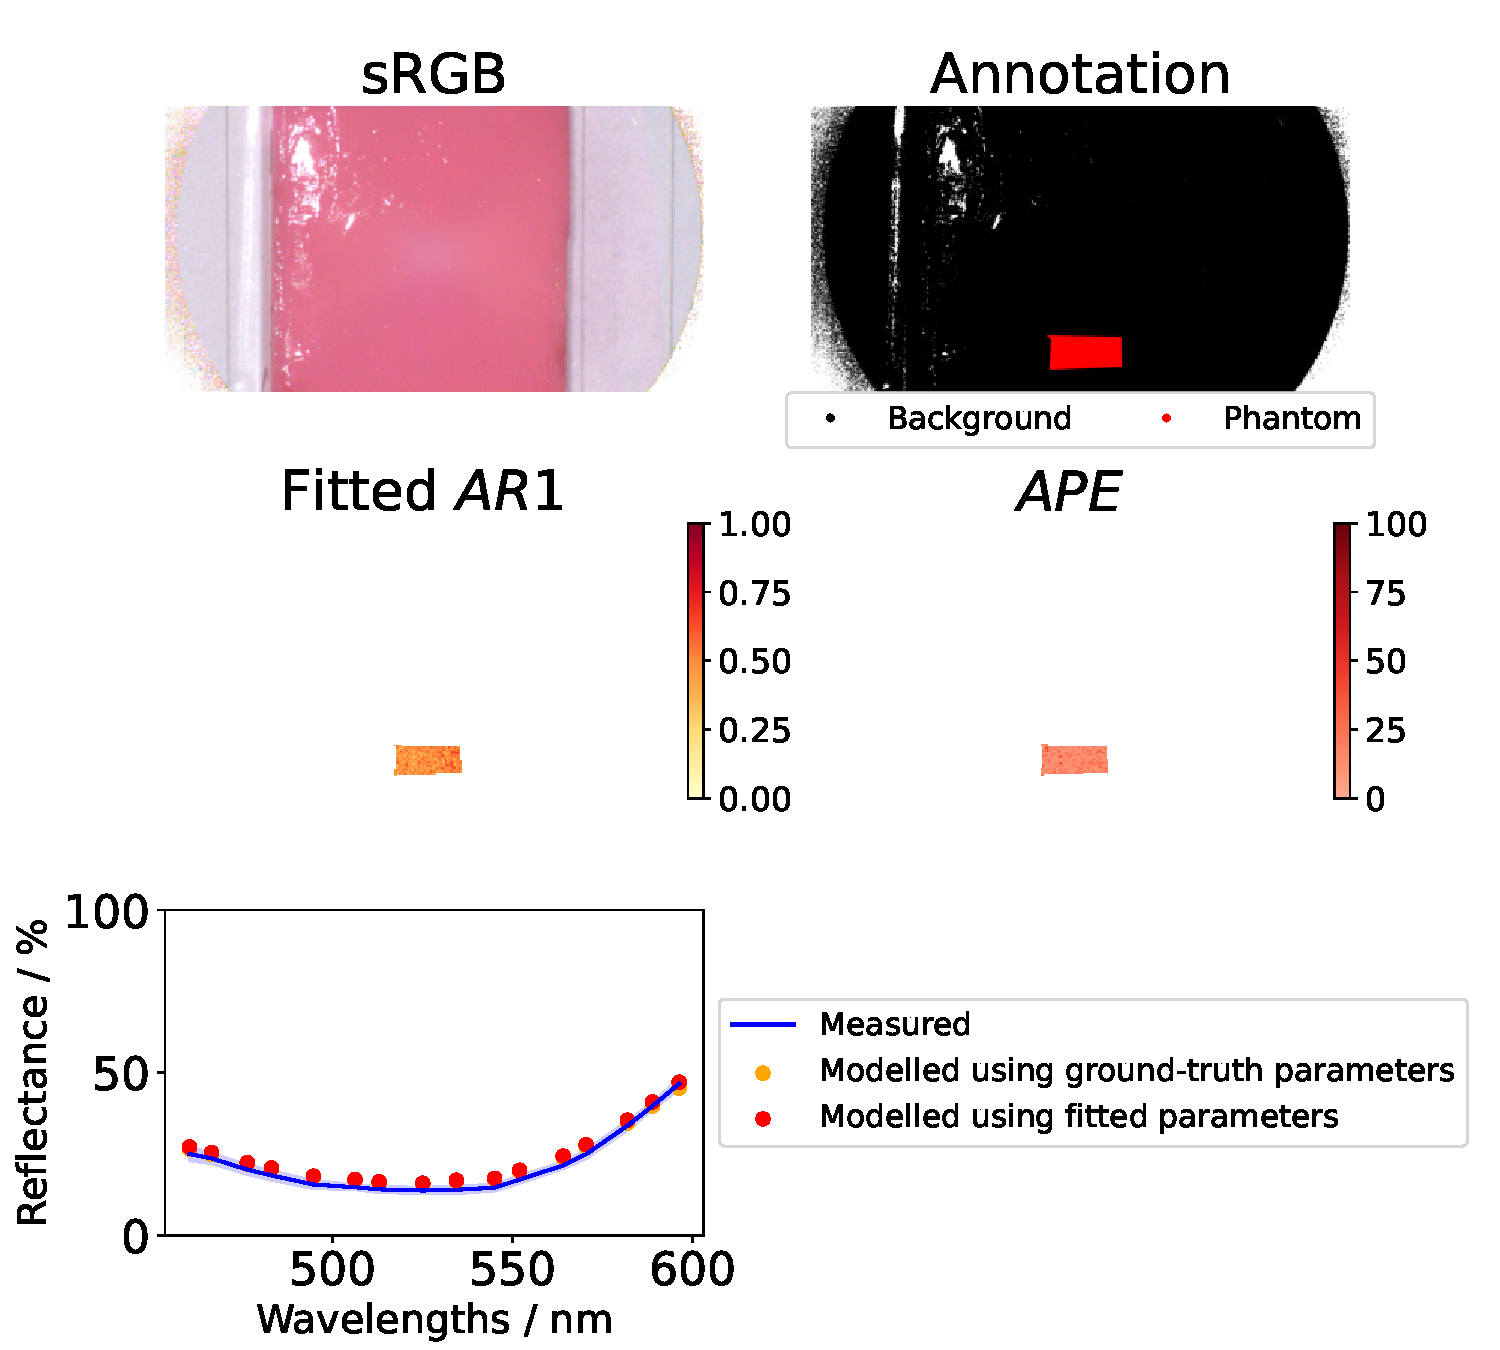
\includegraphics[width=\textwidth]{7_350_Y_OFF_AR1.pdf}
    \caption{Top left shows an sRGB reconstruction of the a gelatin-based phantom where $AR1=0.5$ and $I=3.50\%$ taken with a snapshot HSI camera, where the regions beyond thresholds are shown as white. Top right shows an annotation of the same image. Bottom left shows the fitted $StO_2$ on a pixel-by-pixel basis of the quantitative data using the Yudovsky 2009 single-layer model. Bottom right shows the $APE$ of the fitted $AR1$ of each pixel in the annotated region compared to the ground truth value (0.5).}
    \label{ap:gelatinpbpegQY}
\end{figure}

\begin{figure}[h!]
    \centering 
    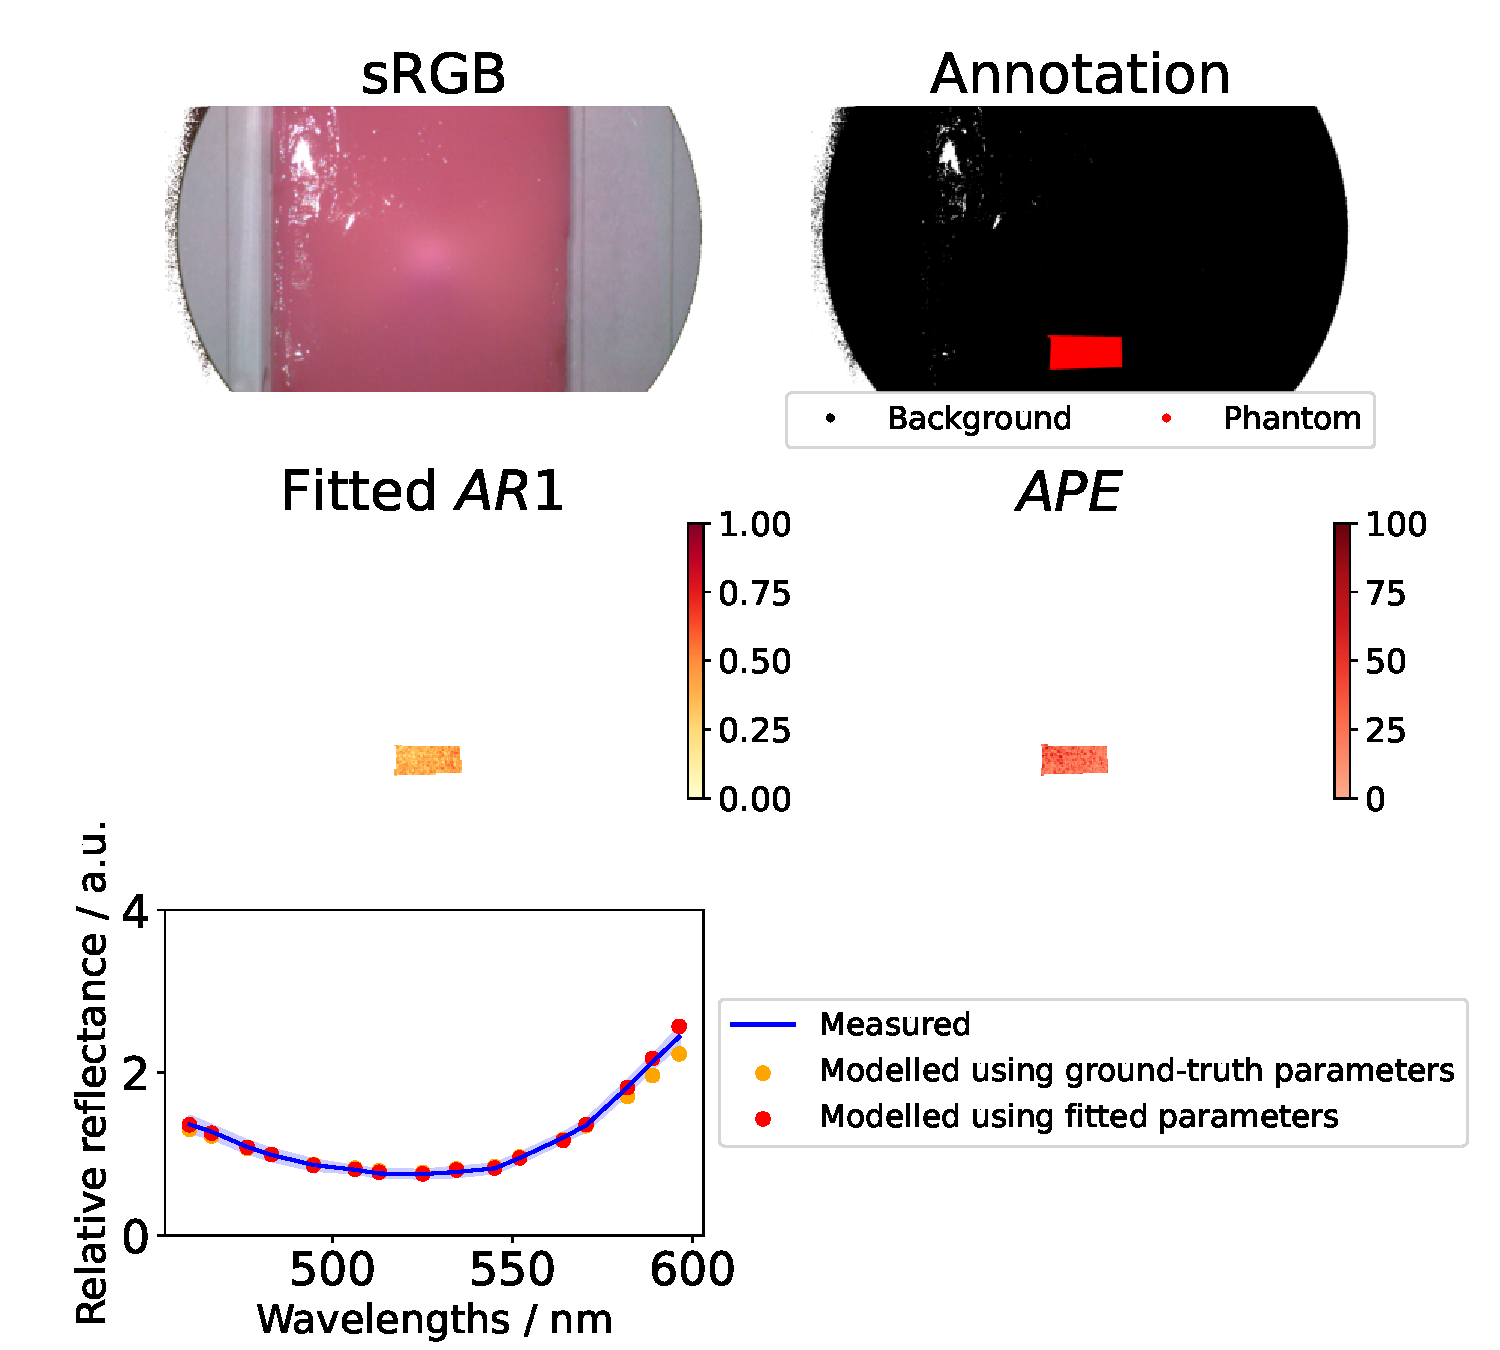
\includegraphics[width=\textwidth]{7_350_J_ON_AR1.pdf}
    \caption{Top left shows an sRGB reconstruction of the a gelatin-based phantom where $AR1=0.5$ and $I=3.50\%$ taken with a snapshot HSI camera, where the regions beyond thresholds are shown as white. Top right shows an annotation of the same image. Bottom left shows the fitted $StO_2$ on a pixel-by-pixel basis of the relative data using the Jacques 1999 single-layer model. Bottom right shows the $APE$ of the fitted $AR1$ of each pixel in the annotated region compared to the ground truth value (0.5).}
    \label{ap:gelatinpbpegRJ}
\end{figure}

\begin{figure}[h!]
    \centering 
    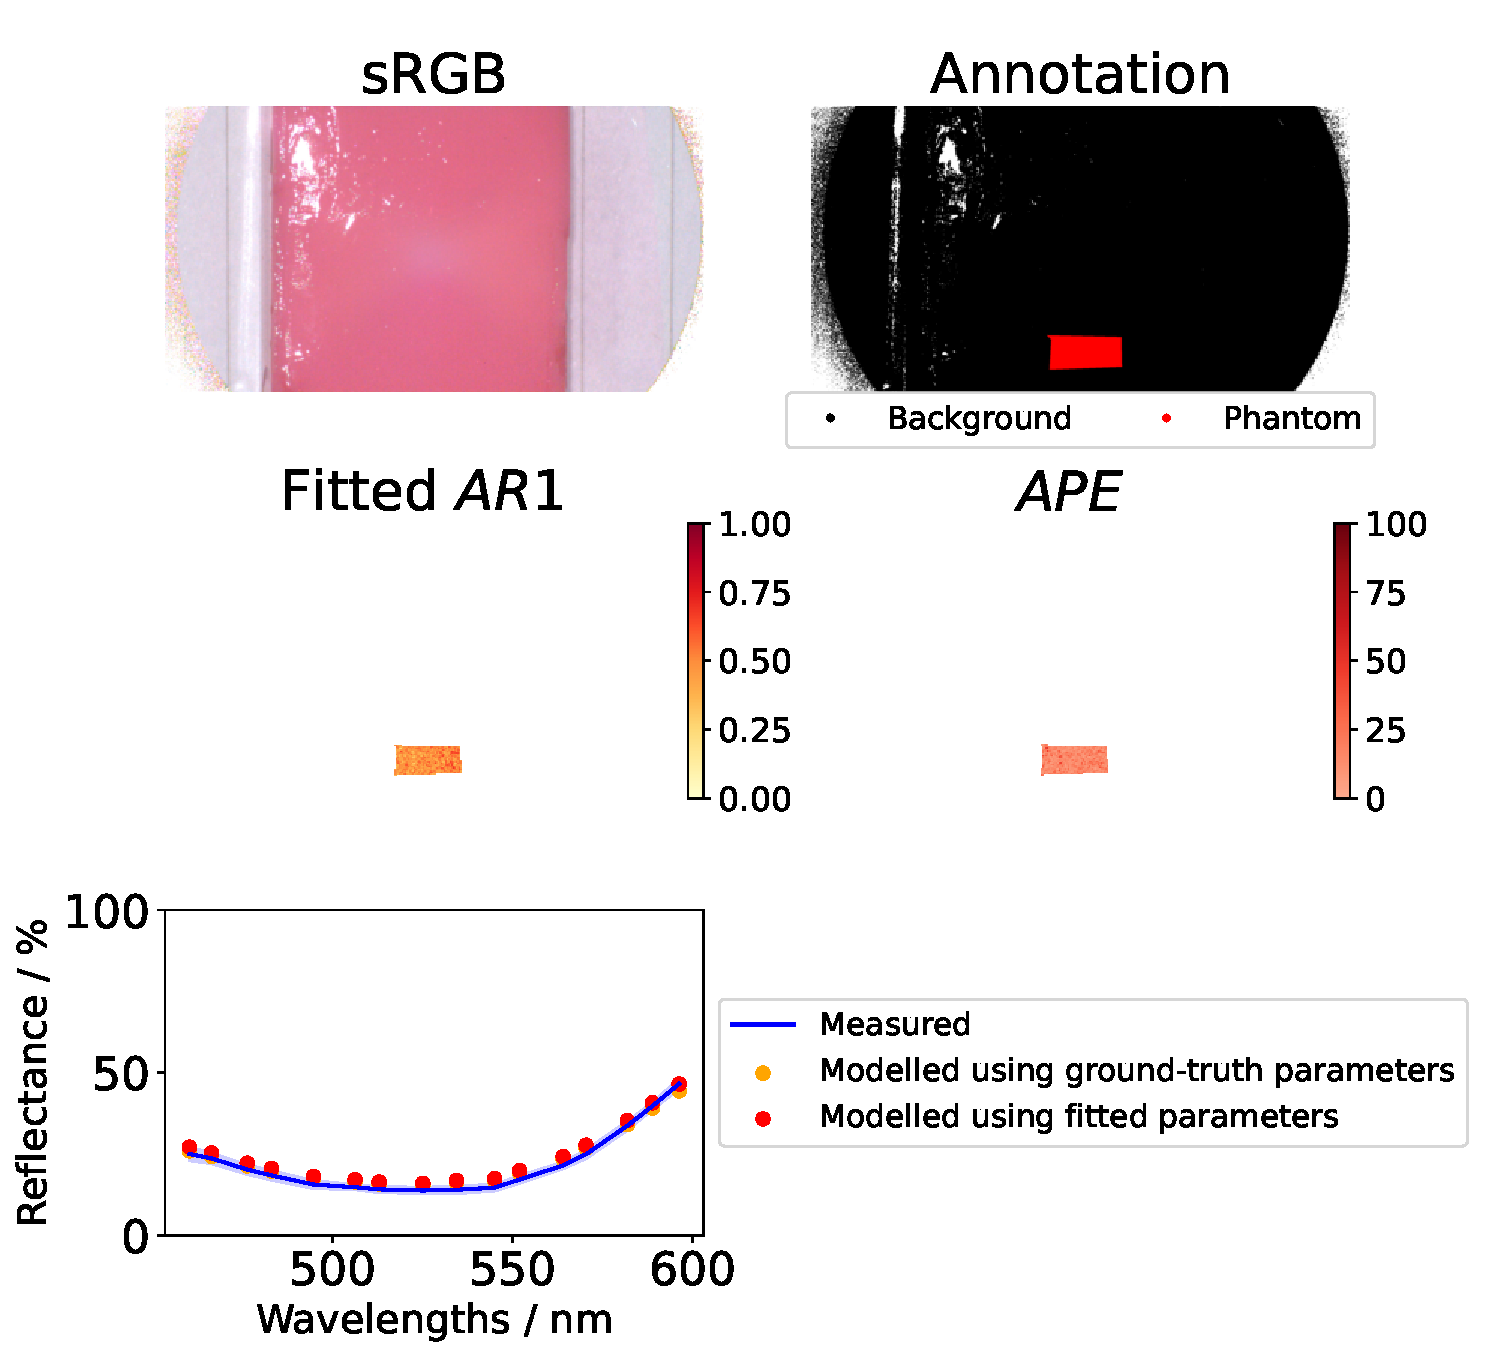
\includegraphics[width=\textwidth]{7_350_J_OFF_AR1.pdf}
    \caption{Top left shows an sRGB reconstruction of the a gelatin-based phantom where $AR1=0.5$ and $I=3.50\%$ taken with a snapshot HSI camera, where the regions beyond thresholds are shown as white. Top right shows an annotation of the same image. Bottom left shows the fitted $StO_2$ on a pixel-by-pixel basis of the quantitative data using the Jacques 1999 single-layer model. Bottom right shows the $APE$ of the fitted $AR1$ of each pixel in the annotated region compared to the ground truth value (0.5).}
    \label{ap:gelatinpbpegQJ}
\end{figure}

\begin{figure}[h!]
    \centering 
    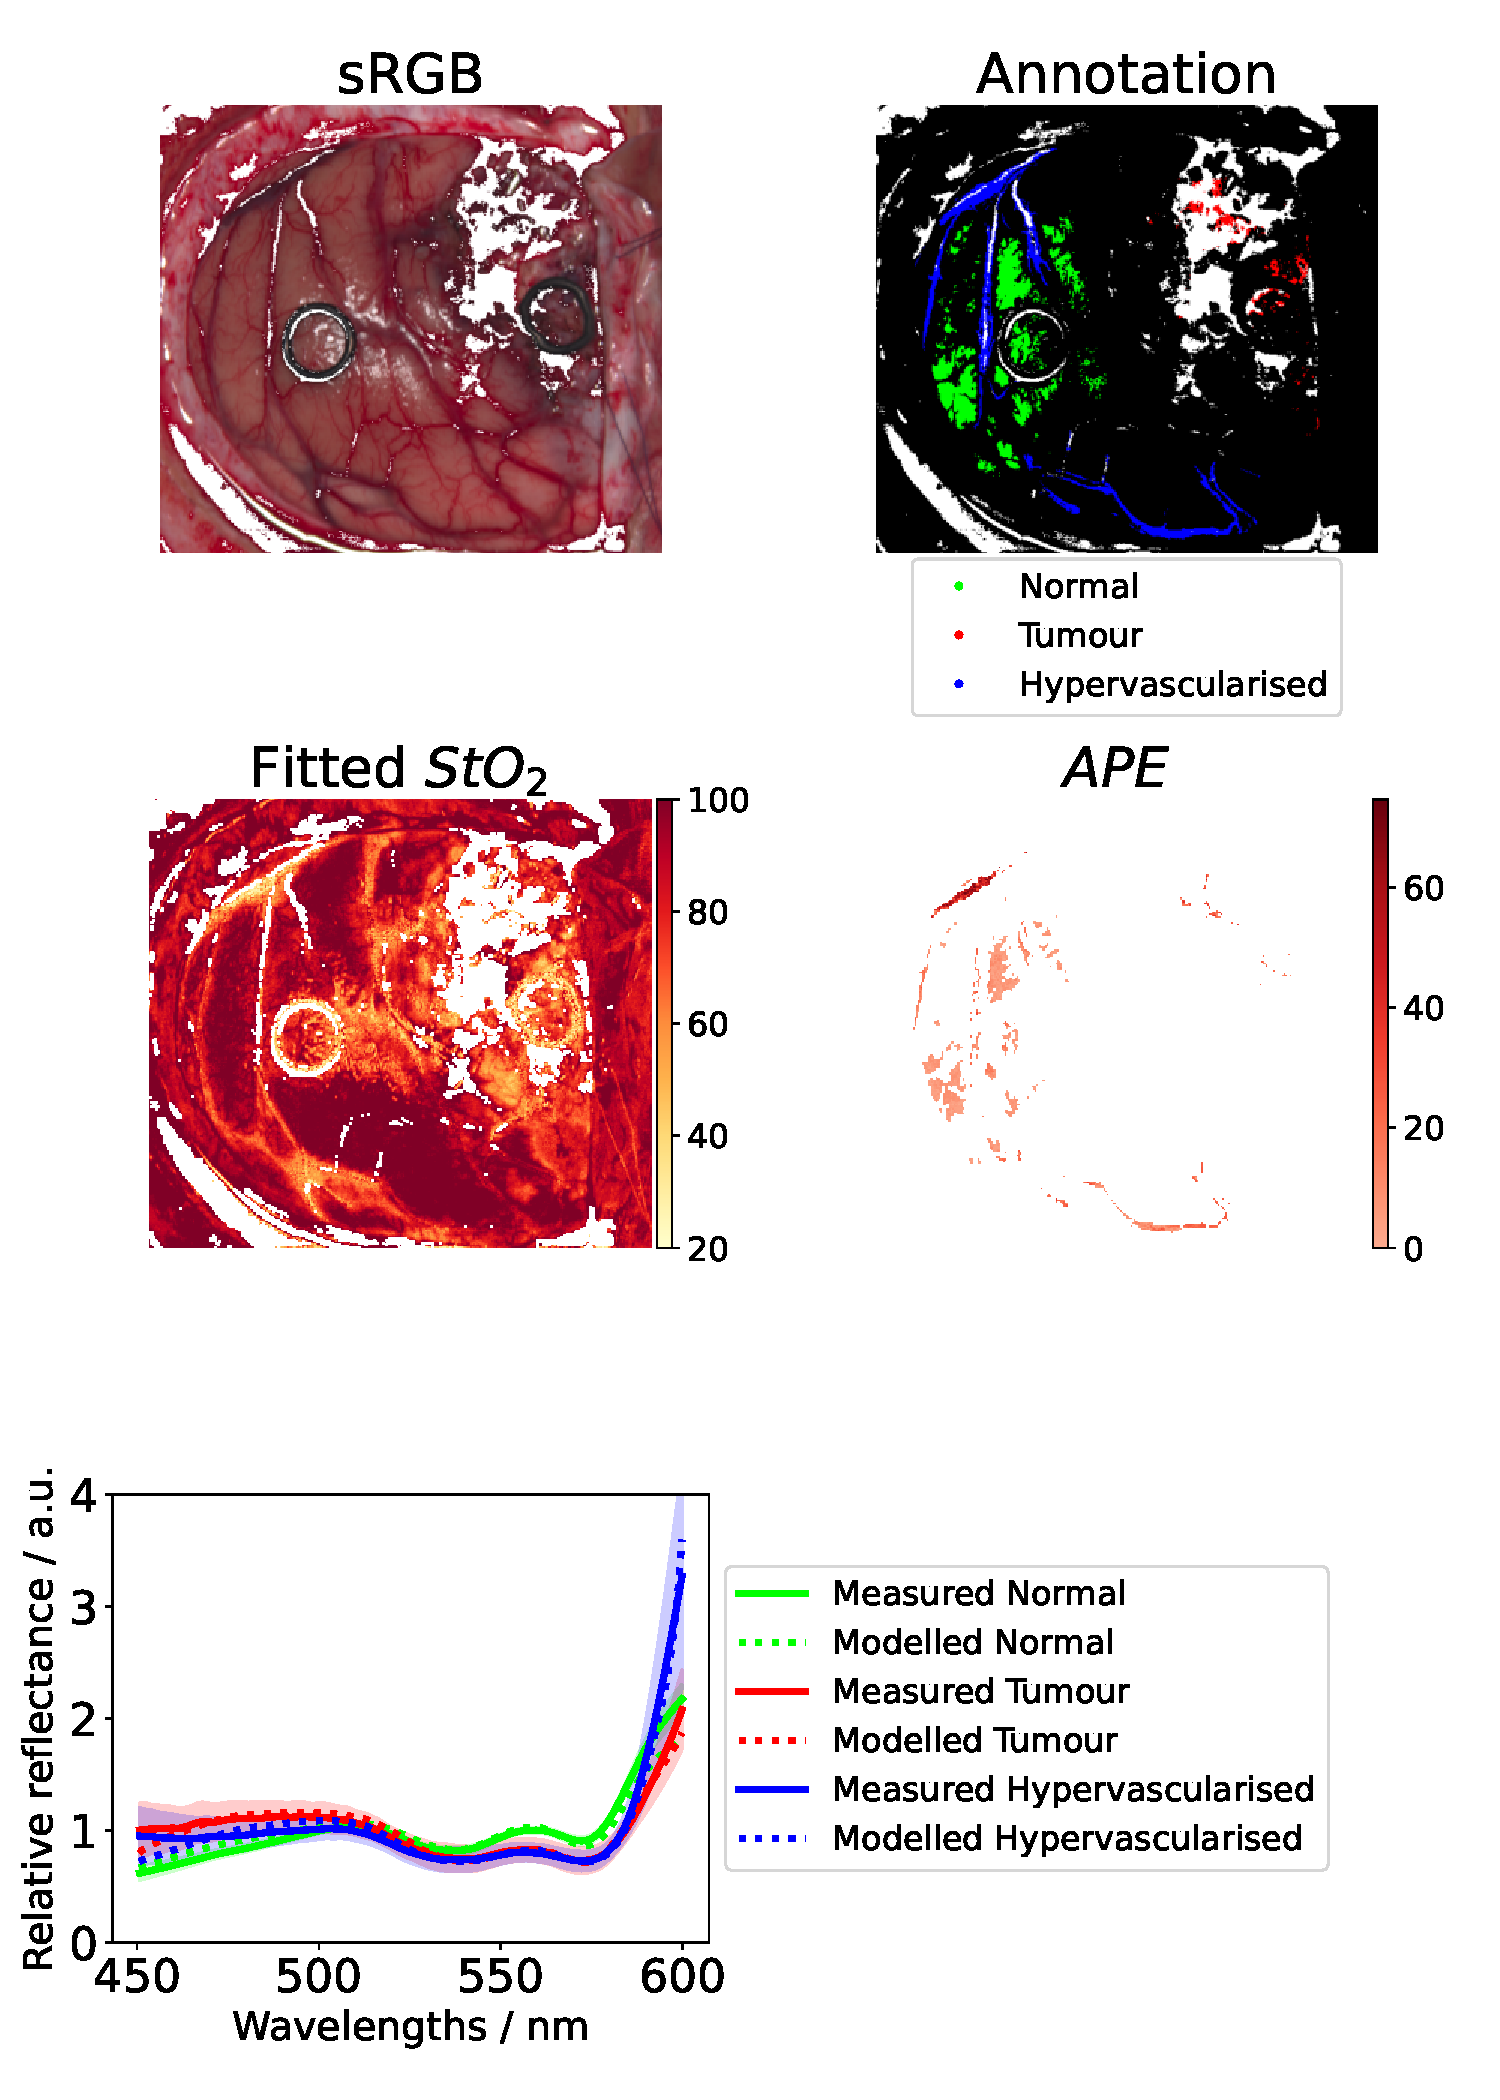
\includegraphics[width=\textwidth]{012-02_StO2_J.pdf}
    \caption{Top left shows an sRGB reconstruction of the HELICoiD image 012-02 with the regions beyond thresholds shown as white. Top right shows an annotation of the same image. Bottom left shows the fitted $StO_2$ on a pixel-by-pixel basis using the Jacques 1999 single-layer model and method 4 (from \ref{sec:NeuroHSIdata}). Bottom right shows the $APE$ of the fitted $StO_2$ of each pixel in each annotated region compared to the fitted $StO_2$ from the mean spectrum of the annotated region.}
    \label{ap:HELICoiDpixelJ}
\end{figure}
\FloatBarrier

\section{Fitting Neurosurgical HSI data with uniform weighting on wavelengths}\label{ap:Chapter5uniform}
\begin{table}[h!]
    \centering
    \caption{The mean (standard deviation) of the fitted physiological parameters when extracted by fitting Yudovsky 2009 single layer (Y) or Jacques 1999 (J) to the relative mean annotated spectra for each tissue type of each image from the HELICoiD dataset using literature (L) or shifted (S) extinction coefficients with uniform weighting of the wavelengths and $n=1.44$. All presented to 3s.f.}
    \begin{tabular}{|ccc|cccc|}
        \hline
        \multirow{2}{*}{Tissue type} & \multirow{2}{*}{Model} & \multirow{2}{*}{Method} & $StO_2$ & $f_{blood}$ & $a$ & $b$ \\
        & & & (\%) & (\%) & ($cm^{-1}$) & (a.u.) \\
        \hline
        \multirow{4}{*}{\shortstack{Hyper-\\vascularised}} & \multirow{2}{*}{Y} & L & 84.0 (20.3) & 2.39 (2.08) & 48.9 (28.9) & 1.72 (1.24) \\
        & & S & 66.7 (27.5) & 3.67 (3.43) & 61.9 (14.8) & 1.50 (0.975) \\
        \cline{2-7}
        & \multirow{2}{*}{J} & L & 78.0 (20.8) & 6.64 (10.7) & 25.9 (27.2) & 1.76 (1.27) \\
        & & S & 55.2 (23.3) & 3.59 (4.42) & 16.0 (21.1) & 1.61 (1.05) \\
        \hline
        \multirow{4}{*}{Normal} & \multirow{2}{*}{Y} & L & 81.9 (22.7) & 0.782 (0.428) & 8.33 (1.85) & 0.318 (0.799) \\
        & & S & 78.0 (23.5) & 0.759 (0.388) & 8.32 (1.80) & 0.327 (0.800) \\
        \cline{2-7}
        & \multirow{2}{*}{J} & L & 84.0 (22.1) & 0.933 (0.701) & 8.46 (2.27) & 0.311 (0.798) \\
        & & S & 80.5 (23.2) & 0.855 (0.553) & 8.52 (2.27) & 0.323 (0.800) \\
        \hline
        \multirow{4}{*}{Tumour} & \multirow{2}{*}{Y} & L & 74.6 (23.6) & 1.06 (0.870) & 13.6 (18.7) & 0.282 (0.377) \\
        & & S & 78.0 (20.3) & 1.85 (2.01) & 26.3 (26.9) & 0.273 (0.324) \\
        \cline{2-7}
        & \multirow{2}{*}{J} & L & 73.9 (24.3) & 1.04 (0.655) & 8.00 (5.24$\times 10^{-15}$) & 0.205 (0.284) \\
        & & S & 75.7 (19.8) & 0.973 (0.545) & 9.94 (4.85) & 0.395 (0.368) \\
        \hline
    \end{tabular}    
    \label{tb:HELICoiDuniform}
\end{table}

\begin{figure}[h!]
    \centering
    \begin{subfigure}{0.49\textwidth}
        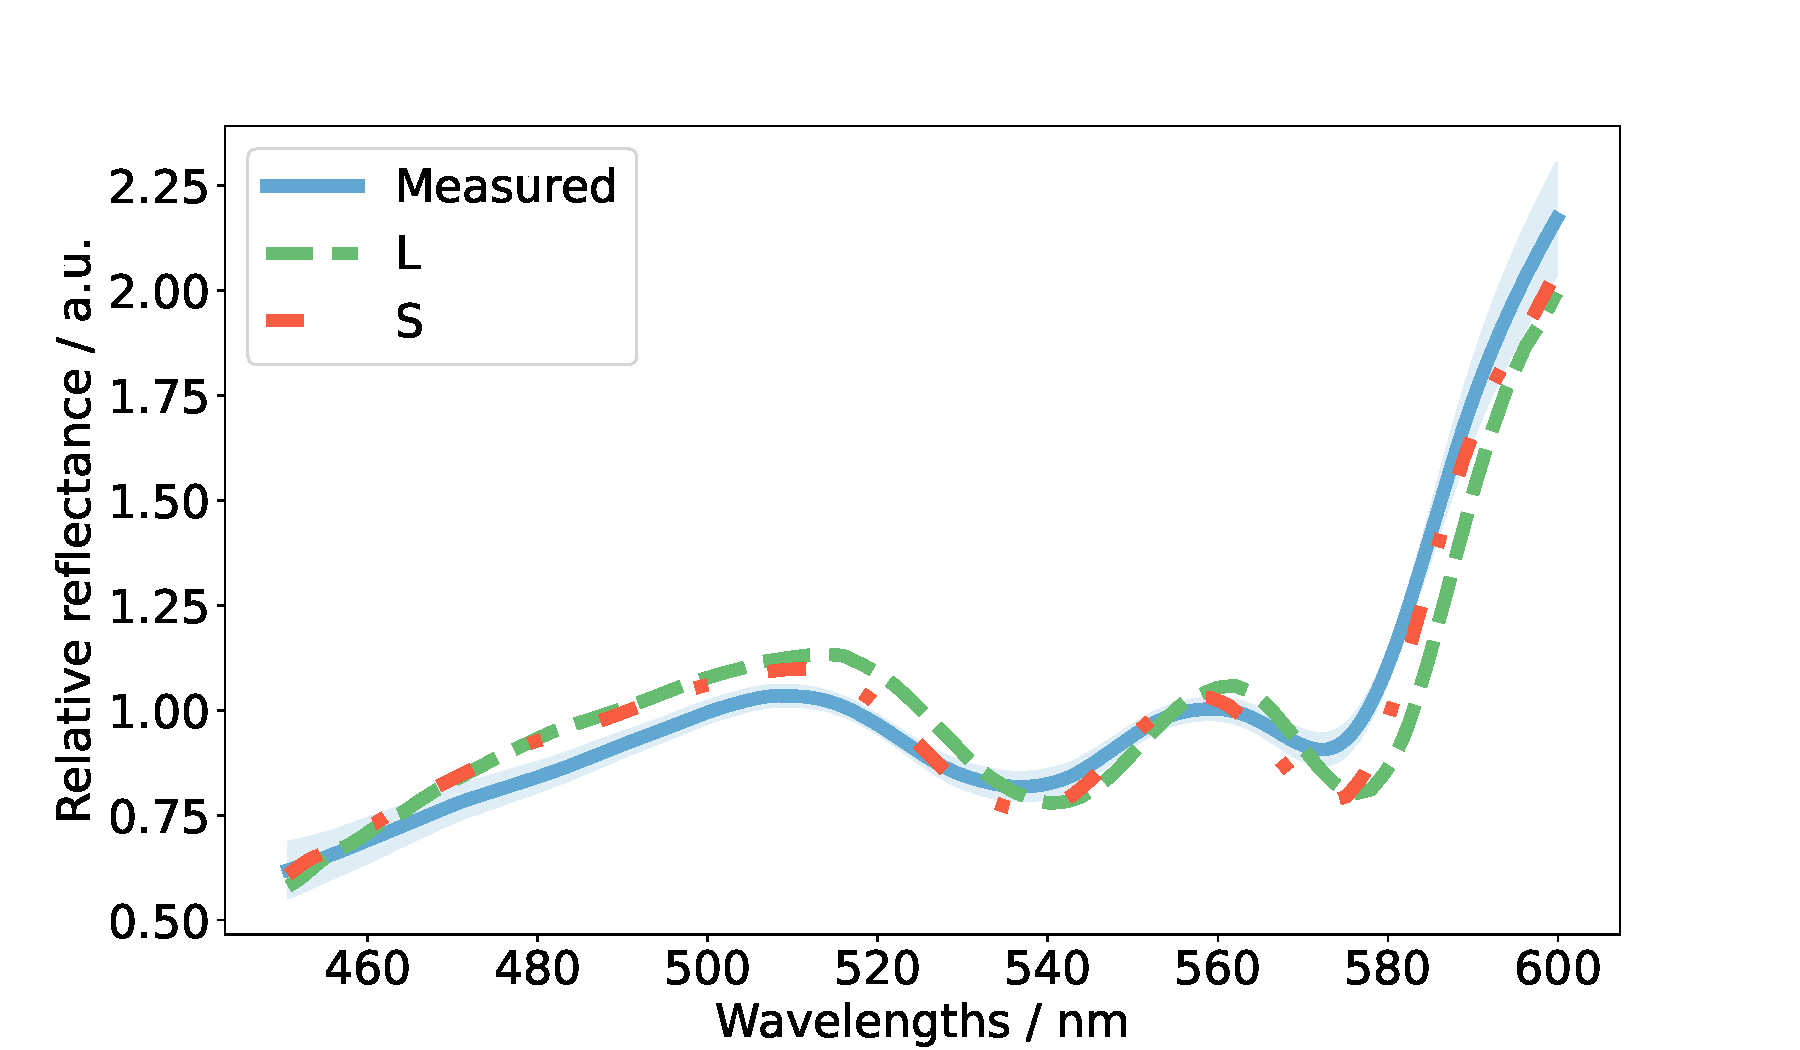
\includegraphics[width=\textwidth]{012-02Normal_spectra_Y_u.pdf}
        \caption{}
        \label{fig:backwardsHSIHeliYuniform}
    \end{subfigure}
    \begin{subfigure}{0.49\textwidth}
        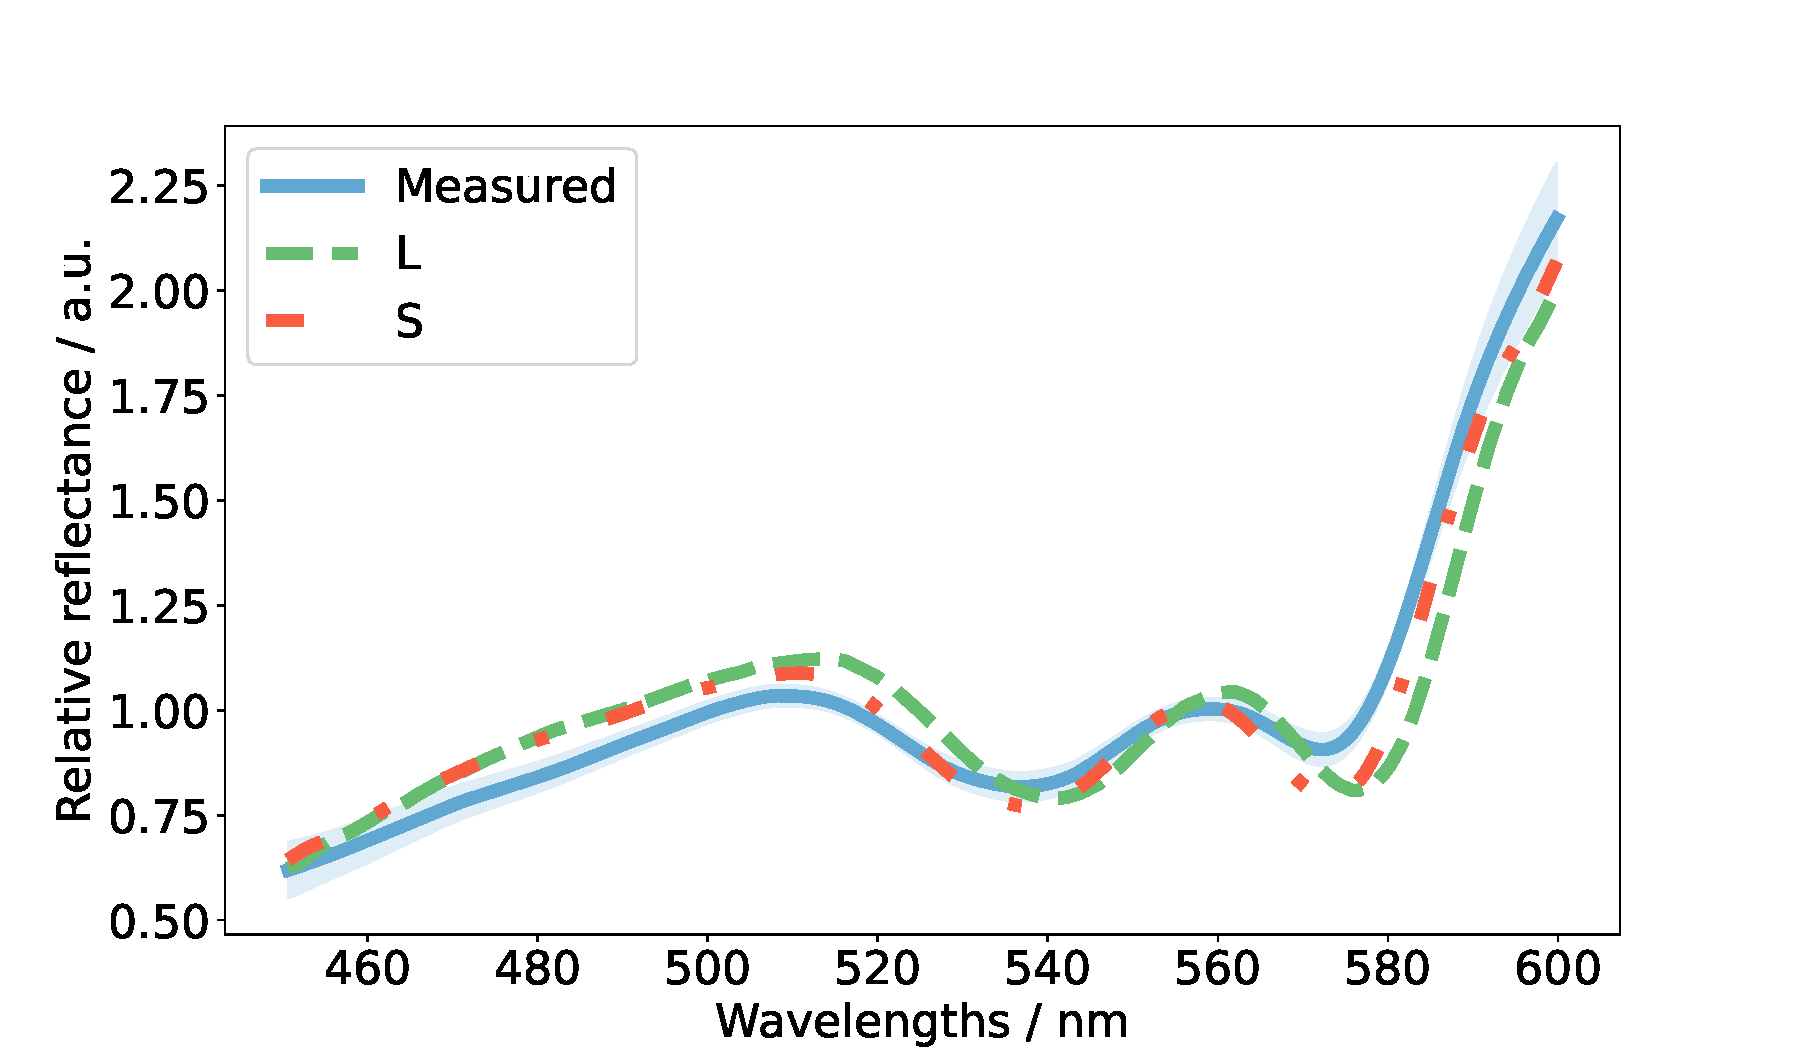
\includegraphics[width=\textwidth]{012-02Normal_spectra_J_u.pdf}
        \caption{}
        \label{fig:backwardsHSIHeliJuniform}
    \end{subfigure}
    \begin{subfigure}{\textwidth}
        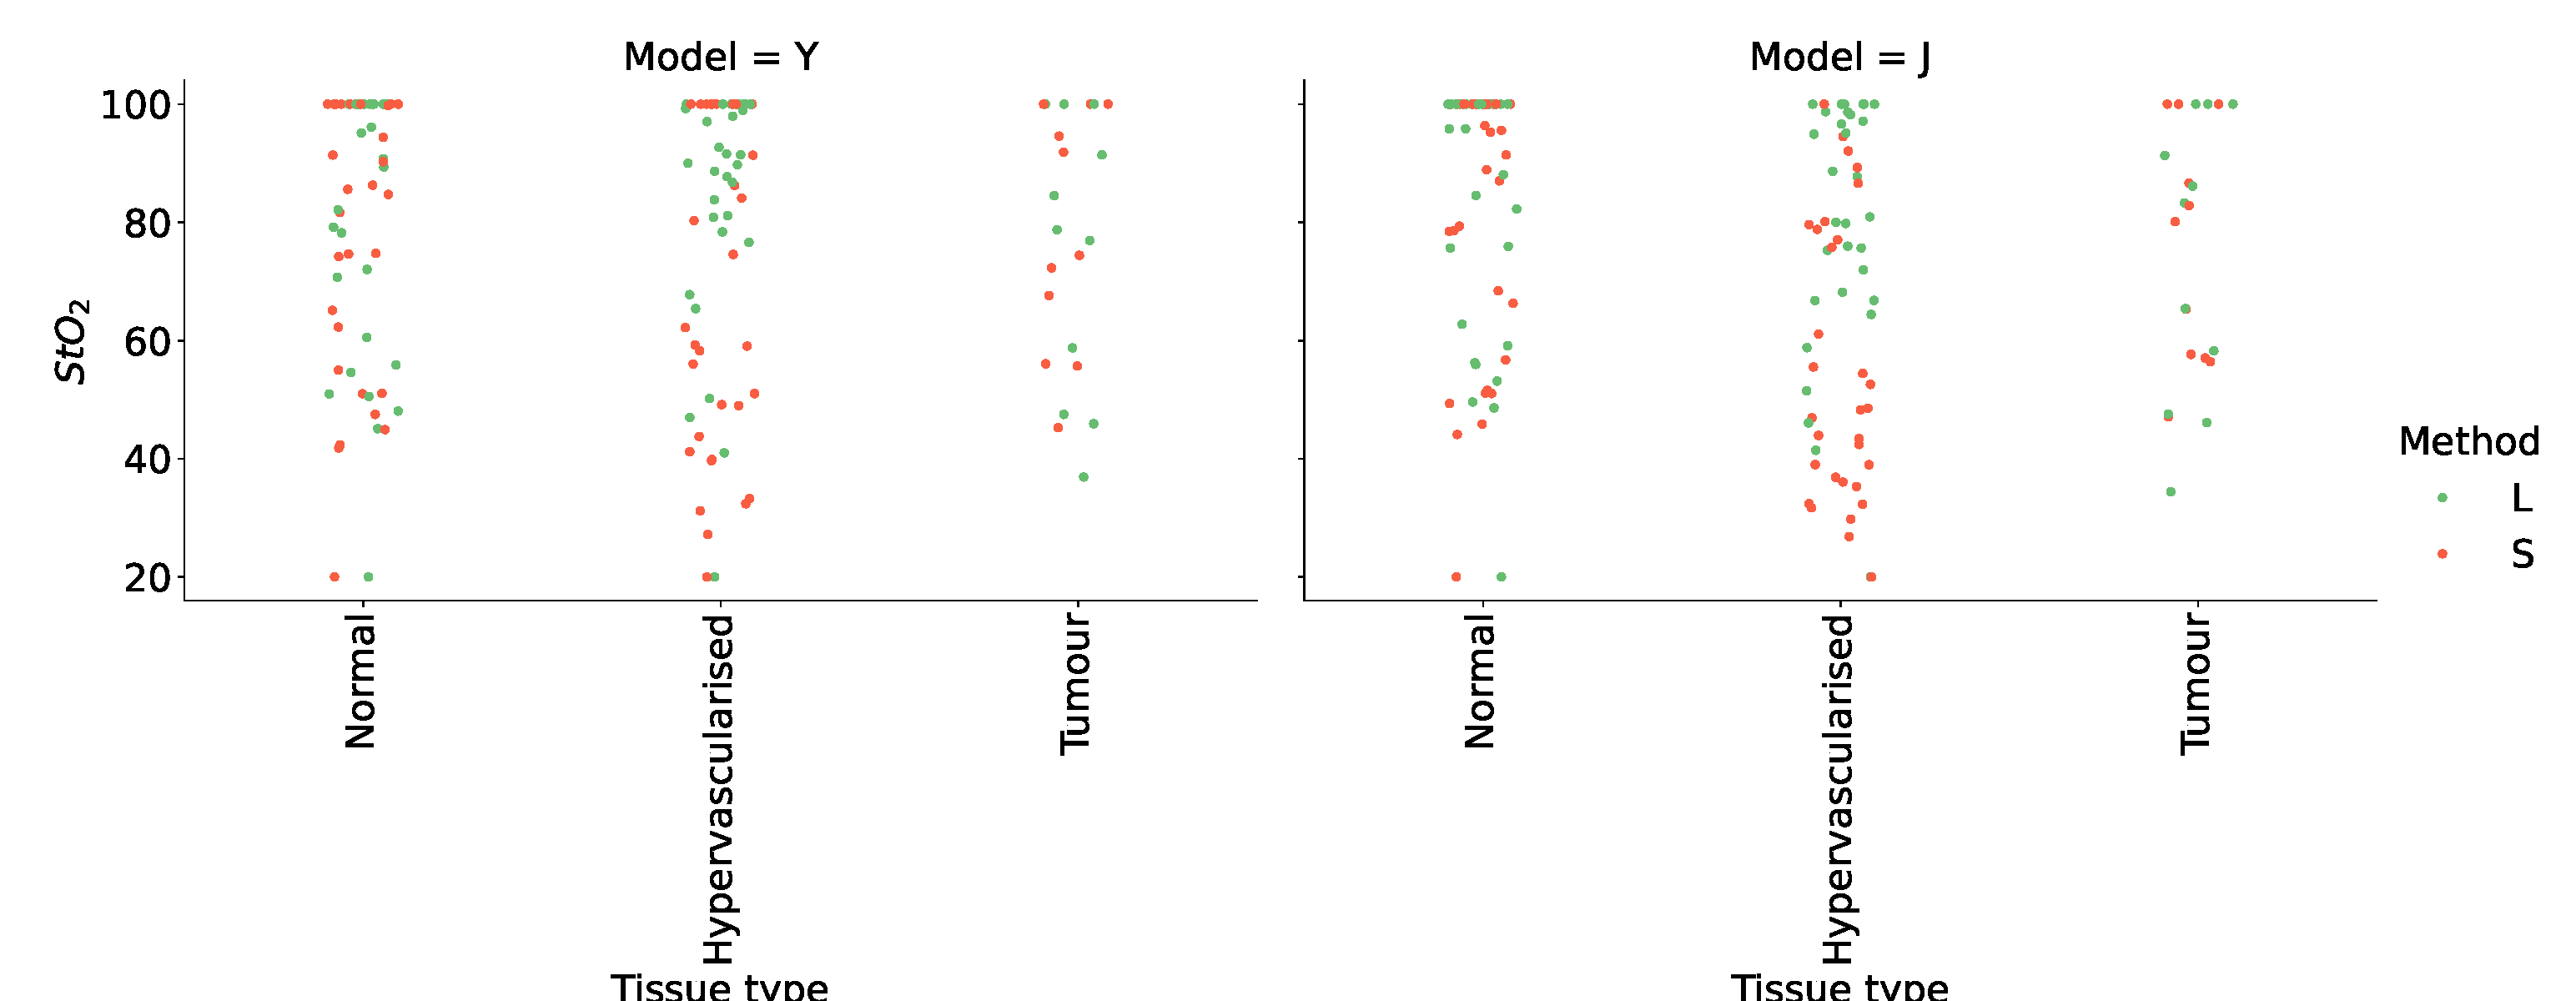
\includegraphics[width=\textwidth]{boxplotsHeli_u.pdf}
        \caption{}
        \label{fig:boxplotsHeliuniform}
    \end{subfigure}
    \caption{An example of the visual fitting quality of the Yudovsky 2009 (\ref{fig:backwardsHSIHeliY}) and Jacques 1999 (\ref{fig:backwardsHSIHeliJ}) single layer models when fitting to the relative mean annotated spectrum ($\pm$1 standard deviation, \textcolor{blue}{blue solid}) of the normal tissue class of HELICoiD image 12-02 using literature (L) or shifted (S) extinction coefficients and a uniform wavelength weighting. The distribution of the fitted physiological parameters retrieved by fitting each model to each relative mean annotated spectrum of the tissue classes of each HELICoiD image is shown in \ref{fig:boxplotsHeli}.}
    \label{fig:HELICoiDannuniform}
\end{figure}